% !TeX root = RJwrapper.tex
\title{\pkg{StratigrapheR}: Concepts for Litholog Generation in R
}
\author{by Sébastien Wouters, Anne-Christine Da Silva, Frédéric Boulvain and Xavier Devleeschouwer}

\maketitle

\abstract{
The \CRANpkg{StratigrapheR} package proposes new concepts for the generation of lithological logs, or lithologs, in R. The generation of lithologs in a scripting environment opens new opportunities for the processing and analysis of stratified geological data. Among the new concepts presented: new plotting and data processing methodologies, new general R functions, and computer-oriented data conventions are provided. The package structure allows for these new concepts to be further improved, which can be done independently by any R user. The current limitations of the package are highlighted, along with the limitations in R for geological data processing, to help identify the best paths for improvements.
}

\section{Introduction}
\CRANpkg{StratigrapheR} is a package implemented in the open-source programming environment R. \textbf{StratigrapheR} endeavors to explore new concepts to process stratified geological data. These concepts are provided to answer a major difficulty posed by such data; namely a large amount of field observations of varied nature, sometimes localized and small-scale, can carry information on large-scale processes. Visualizing the relevant observations all at once is therefore difficult. The usual answer to this problem in successions of stratified rocks is to report observations in a schematic form: the lithological log, or litholog (e.g., Fig.~\ref{figure:drawnlog}). The litholog is an essential tool in sedimentology and stratigraphy and proves to be equally invaluable in other fields such as volcanology, igneous petrology, or paleontology. Ideally, any data contained in a litholog should be available in a reproducible form. Therefore, the challenge at hand is what we would call "from art to useful data"; how can we best extract and/or process the information contained in a litholog, designed to be as visually informative as possible (see again Fig.~\ref{figure:drawnlog}).
\begin{figure}[htbp]
	\centering
	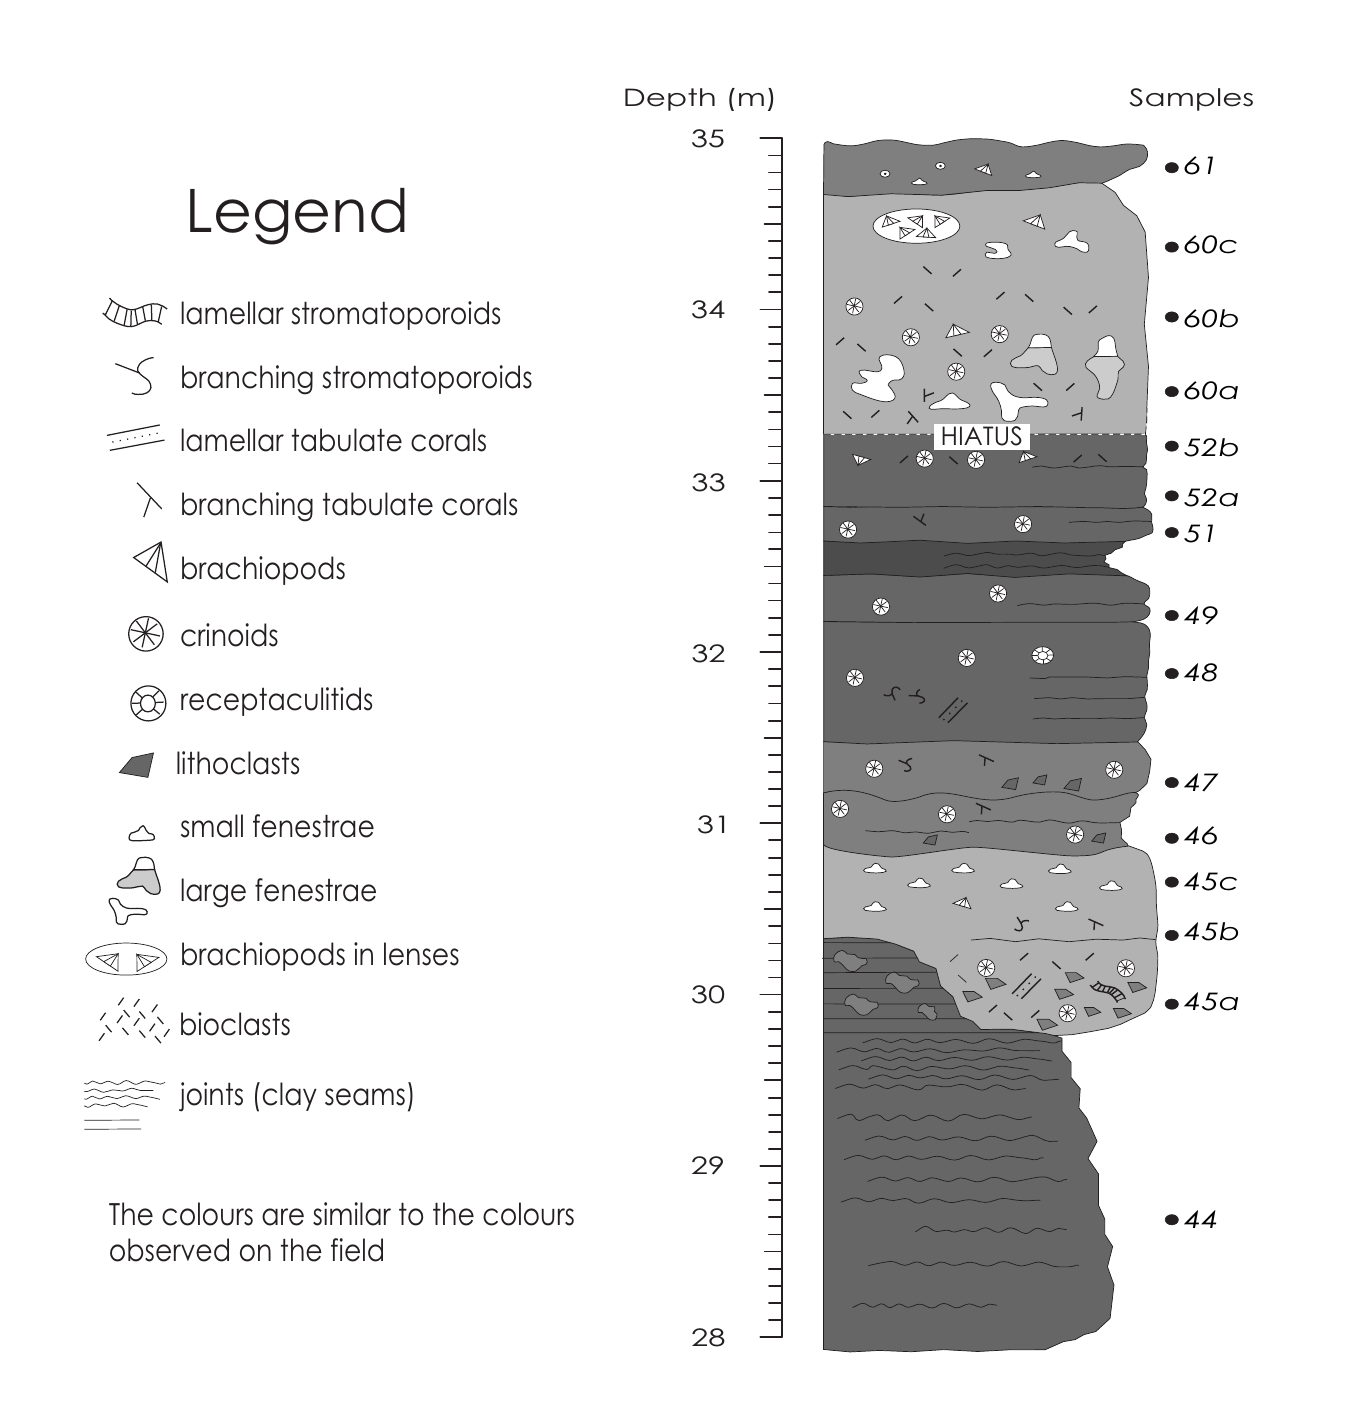
\includegraphics[width=105mm]{Courbe litho SW 3}
	\caption{Example of a computer-drawn litholog of calcareous rocks, modified from \citet{humblet_sedimentology_2000} using vector graphics software (e.g., Inkscape, CorelDRAW, or Adobe Illustrator).}
	\label{figure:drawnlog}
\end{figure}

 Lithologs can be hand-drawn, computer-drawn, or generated via ad hoc software tools. Drawn figures can have unlimited precision and personalization. They are, however, time-consuming to produce and ill-adapted for the extraction of data for further numerical analysis. Moreover, any modification to drawn lithologs has to be performed manually. Ad hoc software tools such as the open-source \href{http://www.sedlog.com/}{SedLog} program \citep{zervas_sedlog_2009} or the \CRANpkg{SDAR} R package \citep{ortiz_sdar_2019} propose a solution to such short-comings by generating lithologs from geological data provided in a text format. The most common text format is the American Standard Code for Information Interchange -ASCII-. ASCII is used for the SedLog data format and for the Log ASCII Standard -LAS- \citep{heslop_log_1999}. The latter (LAS) is the data format used by the \textbf{SDAR} package. 
 
 A major advantage of ad hoc software tools is that any change in the data can automatically lead to an update in the display of the litholog. However, ad hoc software tools only permit a certain amount of personalization. The graphical output of ad hoc software tools, which can be obtained in vector graphics format (e.g., in the Scalable Vector Graphics [SVG] format), has to be post-processed in vector graphics software to add elements that are not supported by the data format. In SedLog, for instance, to add plots next to the litholog (i.e., to visualize quantified analytical values and their relation to the lithological features) the plots need to be generated separately and then added manually along the litholog in vector graphics software. SedLog does permit a certain amount of personalization, but only for the lithological symbology, by giving the user the option of adding self-made symbology (e.g., to show the position of paleontological or sedimentological features). In the \textbf{SDAR} package, the only data automatically displayable are Gamma Ray spectrometry values, and the symbology (for lithology, fossils, etc.) cannot be personalized. 
 
Generally speaking, the graphical style of the lithologs generated by ad hoc software tools is difficult to personalize entirely. To do so, each functionality has to be modular, which is better done in a scripting language such as R. Yet, the \textbf{SDAR} package, although coded in R, is not modular. All the plotting is made using a single function. Any personalization feature would need to be explicitly coded into that function, which would be a never-ending task. Moreover, ad hoc software tools are difficult to update and improve. Adding new functionalities or maintaining the software for compatibility with new operating systems, for example, usually falls on the shoulders of the developers of that software.

The \textbf{StratigrapheR} package is presented here as a new mean to generate lithologs. It provides a complementary approach to the existing methodologies and circumvents the aforementioned problems. \textbf{StratigrapheR} is designed not around a specific data format but on general tools able to deal with different formats. This opens a way of processing the geological data through a scripting language which has a large potential to evolve. \textbf{StratigrapheR} shows that symbiosis between automation and personalization is achievable for litholog generation. As it stands, the package does not meet the "from art to useful data" challenge entirely. However, it is a proof of concept showing that, despite the artistic nature of lithologs, they can be based on usable digital data, or that conversely, usable data can be extracted from drawn lithologs. 

\textbf{StratigrapheR} is coded in R, which disposes of automated package checks \citep{wickham_r_2015} and is itself updated regularly. This is one mechanism against the inevitable obsolescence of the functionalities. Similarly, as the \textbf{StratigrapheR} package is structured in distinct basic functions, implementing  new functionalities (or updating existing ones) can be done more easily by any user. Furthermore, the processing of geological data, whether to generate lithologs or for any other procedure (among others plotting proxies, applying moving averages on these proxies, or performing spectral analysis), can directly be performed in R (see, for instance, the \CRANpkg{paleotree} package for paleontology \citep{bapst_paleotree_2012}, the \CRANpkg{IsoplotR} package for geochronology \citep{vermeesch_isoplotr_2018}, or the \CRANpkg{hht} \citep{bowman_hilberthuang_2013}, \CRANpkg{astrochron} \citep{meyers_astrochron_2014}, \CRANpkg{biwavelet} \citep{gouhier_r_2019} and \CRANpkg{DecomposeR} \citep{wouters_decomposer_2020} packages for spectral analysis). This means that the entire data treatment and visualization could be performed in a single scripting environment: R.

The main concepts for the use of \textbf{StratigrapheR} are presented in this paper. The current limitations of \textbf{StratigrapheR} and R for the processing of geological data are also highlighted to give an idea of the obstacles that the future developers will need to overcome to make R a better tool for geological data processing. Throughout the paper, examples are provided on how to make lithologs and how to process geological data. They can be run in R (you can download R \href{https://www.r-project.org/}{here}); the current version of \textbf{StratigrapheR} (1.2.3) works only on R 4.0 or higher versions. A GitHub repository is available at \href{https://github.com/sewouter/StratigrapheR}{https://github.com/sewouter/StratigrapheR}, where outside users can suggest improvements and provide feedback. The free \href{https://rstudio.com/products/rstudio/#rstudio-desktop}{RStudio} interface is advised to use \textbf{StratigrapheR} in the R environment. The \textbf{StratigrapheR} package can be installed by typing:

\begin{example}
install.packages("StratigrapheR")
\end{example}

To be used, the \textbf{StratigrapheR} package has to be loaded each time R or RStudio are opened, via the following code:

\begin{example}
library(StratigrapheR)
\end{example}

\section{Data importation and processing}

Data of any form can easily be imported using basic R functions, such as \code{read.table()} or \code{readLines()} for text files. Excel files can be downloaded using, for instance, the \code{read.xlsx()} function from the \CRANpkg{xlsx} package \citep{dragulescu_xlsx_2020}. We advise putting any tabular data into data frame form (i.e., a table), which can be done via the \code{data.frame()} function.

As stratigraphic data can be found in an interval form (e.g., a specific strata between 25 and 30 m in a record, or the Jurassic between ca. 200 and ca. 145 million years ago), a formal scheme to deal with such data is provided: the 'lim' object (named after the \code{xlim} and \code{ylim} parameters that define the boundaries of plots in common R graphical functions) and a suite of functions that are associated to lim objects. The idea is to set a logical data format for intervals and to be able to manipulate these intervals in R. The lim objects are made via the \code{as.lim()} function by providing boundaries in the form of the \code{l} and \code{r} arguments, which respectively stand for left and right boundaries. The actual order of the boundaries is irrelevant to avoid unnecessary data cleaning (which is the reason why 'left' and 'right' were chosen as a convention rather than 'up' and 'down'). Each interval can be identified using the \code{id} argument. Providing the upper and lower boundaries allows taking gaps into account in lithologs, contrary to simply providing the thickness of layers (also called beds). Whether the boundaries are included in the interval can be determined via the \code{b} argument, which defines the boundary rules. This is an abstract feature, especially for geology purposes, because it is usually of negligible importance whether the infinitesimal position of a boundary is included in a given interval. However, taking this into account is critical to explicitly describe the behavior of intervals. This can be used, for instance, to assign an interval to a sample located at the common boundary between two intervals that do not overlap otherwise. By providing a boundary rule, it can be explicitly assigned to only one of the two intervals, none of them, or both of them. The boundary rule is expressed by characters, and can be set to \code{"[]"} (or \code{"closed"}) to include both boundary points, \code{"]["} (or \code{"()"}, and \code{"open"}) to exclude both boundary points, \code{"[["} (or \code{"[)"}, \code{"right-open"} and \code{"left-closed"}) to include only the left boundary point, and \code{"]]"} (or \code{"(]"}, \code{"left-open", and "right-closed")} to include only the right boundary point. The left element (e.g., the \code{[} of \code{"[]"}) stands for the left boundary (not necessarily the lowest one), while the right element (e.g., the \code{]} of \code{"[]"}) stands for the right boundary (not necessarily the highest one). We illustrate how to visualize intervals with the following code (note: graphics generated by code in the article are shown directly after the code that generates them):

\begin{example}
interval <- as.lim(l = c(0,1,2), r = c(0.5,2,2.5),   # Make a lim object
                   id = c("Int. 1","Int.2","Int.3"))
                   
interval  # print what is in the lim object
#> $l
#> [1] 0 1 2
#> $r
#> [1] 0.5 2.0 2.5
#> $id
#> [1] "Int. 1" "Int.2"  "Int.3" 
#> $b
#> [1] "[]" "[]" "[]"

# Visualization of the lim object 
plot.new()
plot.window(ylim = c(-0.5, 2.5), xlim = c(0, 2.5))
axis(3, pos = 1.5, las = 1)

infobar(ymin = 0, ymax = 1, xmin = interval$l, xmax = interval$r, 
        labels = c(interval$id), srt = 0)
\end{example}

\begin{figure}[H]
	\centering
	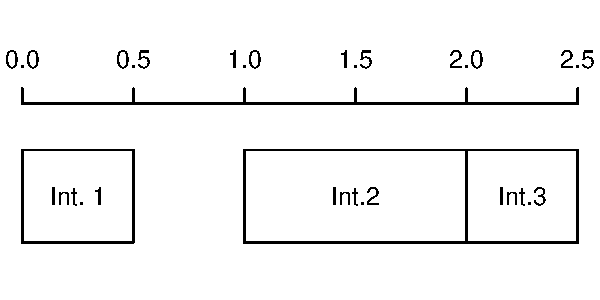
\includegraphics[width=70mm]{int1}
\end{figure}
	
Functions are provided to characterize the relationships of intervals with each other: \code{are.lim.nonunique()} checks whether the intervals are of non-zero thickness (e.g., unlike [1,1]), \code{are.lim.nonadjacent()} checks if the intervals do not share any adjacent boundaries, and \code{are.lim.distinct()} checks whether the intervals are not overlapping. The \code{simp.lim()} function is provided to merge adjacent and/or overlapping intervals having identical IDs. The \code{flip.lim()} function is provided to find the complementary intervals of a set of intervals (i.e., the gaps). The \code{mid.lim()} function provides a way to define intervals in between data points. If all different intervals are strictly non-overlapping for all values (for instance, the intervals [0,20[ and [20, 100] are non-overlapping and therefore 20 is uniquely represented by the second interval), the \code{in.lim()} function can be used to find which values belong to which respective intervals. Typically, such functions can be used to craft stratigraphic intervals (such as magnetochrons or stages) and determine the beds or samples that are in or outside them.

\section{General plotting considerations}

The first challenge when plotting a litholog is its size: a litholog needs to be detailed at a small scale (typically at the centimeter scale for high precision) while spanning the entirety of a record (up to hundreds of meters). This makes lithologs sometimes quite extended. This is problematic considering that the classical R graphic window is not adapted to visualize anything exceeding the size of the computer screen. To remedy this problem, the \code{pdfDisplay()} function is here introduced, which draws plots directly in a PDF (Portable Document File) document and opens it in the computer’s default PDF reader. This PDF document can have any size desired by the user, and therefore, allows visualizing all the details of a very long litholog. This is illustrated by the code here below, which draws a vertically standing stickman. Depending on the screen, this vertical stickman could be difficult to visualize without \code{pdfDisplay()}.

To avoid having to close the PDF reader at each change of the plot (as most PDF readers do not permit changes to the PDF file while it is displayed), each new PDF can be named differently: each new document version will have its name be followed by '\_(i)', where i is the version number (e.g., test\_(1).pdf, test\_(2).pdf, etc.). This practice is here referred as \emph{tracking} the version number. It is noteworthy to cite the free \href{https://www.sumatrapdfreader.org/free-pdf-reader.html}{Sumatra PDF} software, which is available for Windows operating systems, and lets PDF files be modified while still displaying them without the trick of having to change the file name. In that case, the tracking of the version numbers can be canceled by setting the \code{track} parameter to \code{FALSE}. PDF files generated by \code{pdfDisplay()} can easily be imported into vector graphics software. The \code{pdfDisplay()} function also allows for the direct generation of an SVG file. \code{pdfDisplay()} is a wrapper of the more basic \code{pdf()} function (i.e., its code is based on the \code{pdf()} function); other PDF generating functions could be used interchangeably.

To make plots starting from an empty background, we advise using the \code{plot.new()} and \code{plot.window()} functions, which are of lower level (i.e., more basic) than the \code{plot()} function. They are used to create a completely empty plotting environment in which to add the litholog. To add axes, the \code{axis()} function is a versatile tool, which can be replaced by the \code{minorAxis()} function provided in \textbf{StratigrapheR} to add minor axis ticks. The \code{minorAxis()} function is itself a wrapper of the \code{axis()} function.

\begin{example}
graphical_function <- function() # Graphical function needed by pdfDisplay 
{
   opar <- par()$mar # Save initial graphical parameters
   par(mar = c(0,3,0,1)) # Change the margins of the plot
	
   plot.new() # Open a new plot
   plot.window(xlim = c(-0.2, 1.2), ylim = c(-5, 1)) # Define plot coordinates
   minorAxis(2, at.maj = seq(-5, 1, 0.5), n = 5, las = 1) # Add axis
   points(c(0.25, 0.75), c(0.75, 0.75), pch = 19)
   polygon(c(0.1, 0.25, 0.75, 0.9, 0.75, 0.25, NA, 
             0, 0.25, 0.75, 1, 0.75, 0.25),
           c(0.5, 0.25, 0.25, 0.5, 0.4, 0.4, NA,
             0.5, 0, 0, 0.5, 1, 1), lwd = 2)
   lines(x = c(0.5, 0.5, NA, 0, 0.2, 0.5, 0.8, 1, NA, 
               0, 0.2, 0.5, 0.9, 1.2),
         y = c(-0.25, -3, NA, -5, -4, -3, -4, -5, NA, 
               -2.5, -1.5, -1, -0.75, 0.25), lwd = 2)
	      
   par(mar = opar) # Restore initial graphical parameters
}

pdfDisplay(graphical_function(),"graphical_function", width = 3.5, height = 10)
\end{example}

\begin{figure}[H]
	\centering
	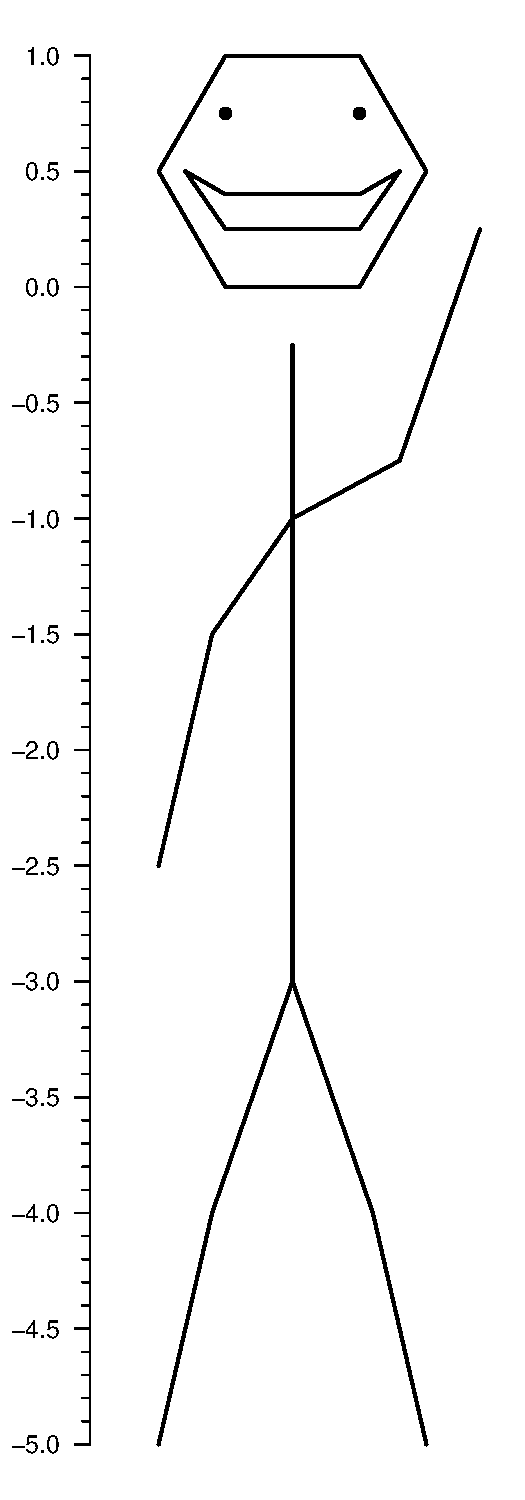
\includegraphics[width=37mm]{graphical_function}
\end{figure}

Adding every element of the lithologs symbology uses a very basic data format for polylines and polygons, which are respectively drawn using the \code{multigons()} and \code{multilines()} functions. These novel functions allow precise control of graphical parameters when drawing multiple polygons and polylines. These functions require an identification argument \code{i}, similar for each point of a single polygon or polyline, and the \code{x} and \code{y} coordinates of each point. The following code shows the use of the \code{multigons()} and \code{multilines()} functions:

\begin{example}
i <- c(rep("A1",6), rep("A2",6), rep("A3",6)) # Polygon IDs
x <- c(1,2,3,3,2,1,2,3,4,4,3,2,3,4,5,5,4,3)   # x coordinates
y <- c(1,2,3,4,5,6,1,2,3,4,5,6,1,2,3,4,5,6)   # y coordinates
	
plot.new()
plot.window(xlim = c(0,6), ylim = c(0,7))

multigons(i, x, y,
          front = "A2", # This gets the polygon A2 in front of all others
          density = c(NA, 5, 10),  # Shading line density
          scol = "grey20", # Shading line color; one value means all polygons
                           # are subject to this graphical parameter
          col = c("black", "grey80", "white"), # Background color
          lwd = 2, # Width of border lines
          slty = 2, slwd = 1) # Shading lines type and width  
\end{example}

\begin{figure}[H]
	\centering
	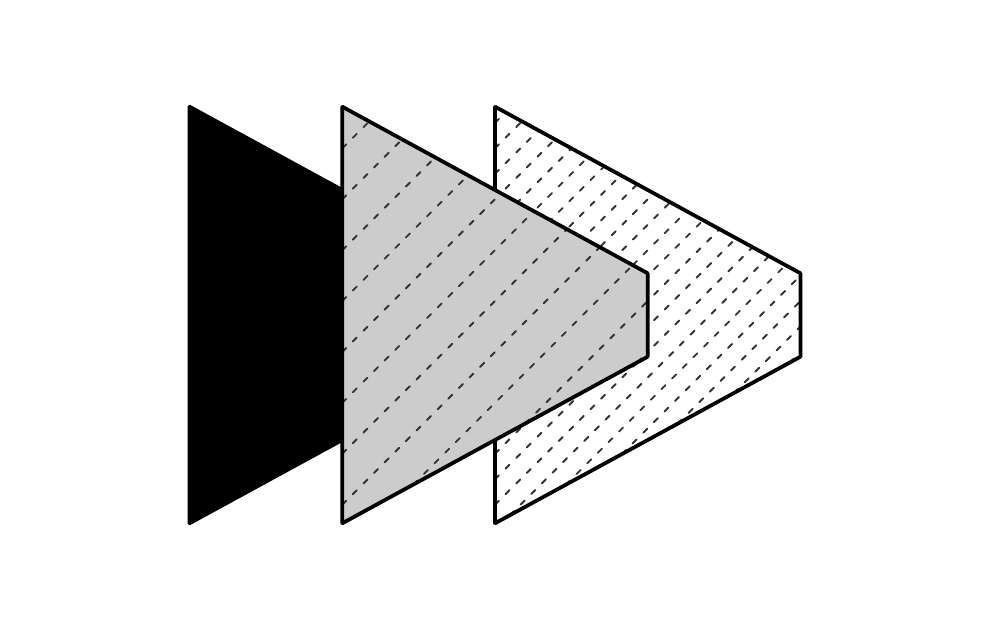
\includegraphics[width=70mm]{multigons}
\end{figure}

\begin{example}
i <- c(rep("A1",6), rep("A2",6), rep("A3",6)) # Lines IDs
x <- c(1,2,3,3,2,1,4,5,6,6,5,4,7,8,9,9,8,7)   # x coordinates
y <- c(1,2,3,4,5,6,1,2,3,4,5,6,1,2,3,4,5,6)   # y coordinates
	
plot.new()
plot.window(xlim = c(0,10), ylim = c(0,7))
	
multilines(i, x, y, 
           j = c("A3", "A1", "A2"),  # j controls the order of the graphical 
                                     # parameters applied to each named line:
           lty =  c(1,2,3), lwd = 2, # e.g., lty = 1 (solid line) is applied  
                                     # to "A3", the line at the right
           type = c("l", "o", "o"), 
           pch = c(NA,21,24), cex = 1, bg = "black")
\end{example}

\begin{figure}[H]
	\centering
	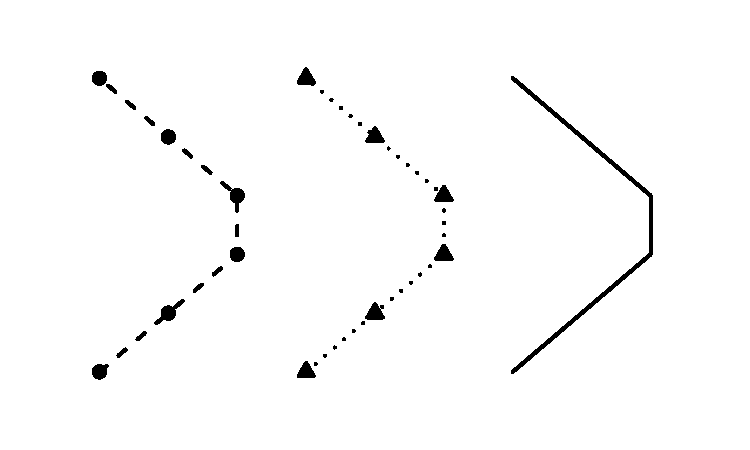
\includegraphics[width=60mm]{multilines}
\end{figure}

The \code{pointsvg()} function is provided in \textbf{StratigrapheR} to import groups of polygons and polylines drawn in vector graphics software, under specific conditions: firstly, the drawing needs to be in SVG format; secondly, the \code{pointsvg()} function is only able to identify objects of class "line", "rect", "polygon", and "polyline" in the SVG file. The reason for this is that only these types of objects are simple lines, and polygons made of nodes linked together by straight lines. This means that \code{pointsvg()} is not able to recognize all the objects present in an SVG file. Furthermore, \code{pointsvg()} only identifies the coordinates of each objects, regroups them into separate polygons and polyline objects, and in which order to plot them. All other graphical parameters, such as color or line thickness, are not taken into account. These parameters have to be specified in the drawing functions. Objects obtained using \code{pointsvg()} on SVG files can be added using the \code{framesvg()} or \code{centresvg()} functions, which respectively add the object within a given frame or center the object on a given point.

\begin{example}
svg.file.directory <- tempfile(fileext = ".svg")     # Creates temporary file
writeLines(example.ammonite.svg, svg.file.directory) # Writes svg in the file

ammonite.drawing <- pointsvg(file = svg.file.directory) # Read svg

plot.new()
plot.window(xlim = c(-2, 5), ylim = c(-2, 2))
axis(1)
axis(2, las = 2)

centresvg(ammonite.drawing,  # Object
          x = c(3,0), y = 0,  # Coordinates for centering
          xfac = 2, yfac = 2,  # Dimension stretching factors
          col = c("grey","white"))  # Graphical parameters
\end{example}

\begin{figure}[H]
	\centering
	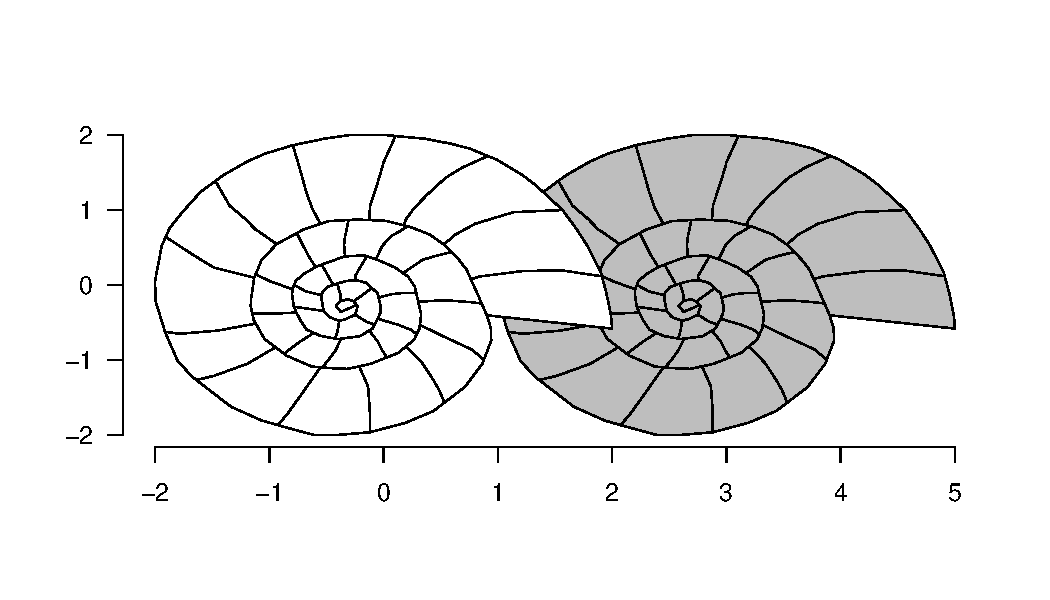
\includegraphics[width=75mm]{ammonite}
\end{figure}

It should be noted that repetitions of the same SVG object can be generated by a single call of the \code{framesvg()} or \code{centersvg()} functions. This facilitates the automation of the litholog generation. Modifications of the SVG objects can also be accomplished using the \code{changesvg()} function, which enables, among other things, to change the order of plotting of the polylines and polygons, remove some of them, or invert the figure in x and/or y. The \code{framesvg()} or \code{centersvg()} can also output the drawing with modified coordinates, which can be plotted using \code{placesvg()} (see, for instance, the code of the last example).

\section{Generating lithologs}

The data to make lithologs can be provided in the form shown in Table \ref{Tab:beds}.

\begin{table}[H]
\centering
\begin{tabular}{*{6}{c}}
	\toprule
	id & l & r & h & colour & litho \\
	\midrule
	B1 & 0 & 1 & 3 & grey &	S \\
	B2 & 1 & 3 & 4 & grey &	L \\
	B3 & 3 & 4 & 5 & black & C \\
	B4 & 4 & 9 & 4 & white & L \\
	B5 & 9 & 11 & 4 & white & L \\
	...&...&...&...&...&... \\
	\bottomrule
\end{tabular}
\caption{Example of a data frame (\code{bed.example} in \textbf{StratigrapheR}) providing information for each bed: id identifies each bed, l and r provide the boundaries, h the hardness, and the color is provided along with a code for lithology (S for shale, L for limestone, C for chert). The only strict convention is that l, r, and h need to be numerical values.}
\label{Tab:beds}
\end{table}

From such data, basic lithologs made of rectangles can be generated as a simple basis. They are the starting point for making more complicated lithologs in \textbf{StratigrapheR}. The coordinates of the points making up the rectangles can be computed through the \code{litholog()} function, which only needs the position of the boundaries of the beds, their 'hardness', and an ID. Text can be added to each bed using the \code{bedtext()} function, which can be used to include the ID or the name of the bed (e.g., id in Table \ref{Tab:beds}).

The output of the \code{litholog()} function can be provided to \code{multigons()} to draw the log. A symbology for different types of rocks (or any other information that the symbology is meant to provide) can be set up using the color fill and the shading. Providing a given symbology for each polygon is performed by joining the table containing the information about each bed to a table attributing symbology to rock type. We advise the use of the \code{left\_join()} function in the \CRANpkg{dplyr} package \citep{wickham_dplyr_2020} for this procedure.

\begin{example}
basic.log <- litholog(l = bed.example$l,  # This creates a data table of
                      r = bed.example$r,  # rectangles coordinates for a
                      h = bed.example$h,  # basic litholog
                      i = bed.example$id) 

legend <- data.frame(litho = c("S", "L", "C"),             # This creates a  
                     col = c("grey30", "grey90", "white"), # data table for   
                     density = c(30, 0,10),                # the symbology
                     angle = c(180, 0, 45), stringsAsFactors = FALSE)
View(legend)               
\end{example}

\begin{figure}[H]
	\centering
	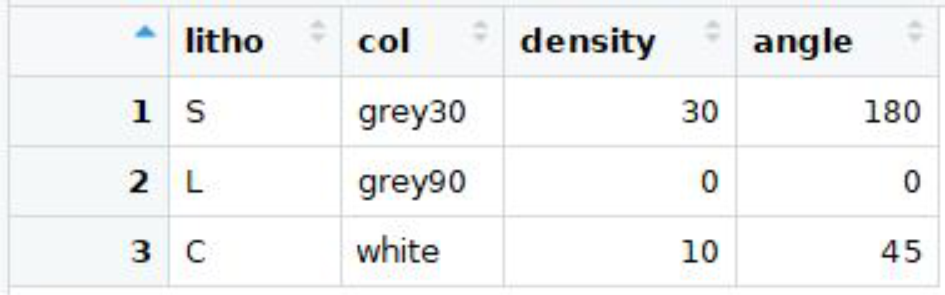
\includegraphics[width=75mm]{Legend table}
\end{figure}

\begin{example}
# left_join in the dplyr package merges the symbology with the table of beds:
bed.legend <- dplyr::left_join(bed.example,legend, by = "litho")

View(bed.legend)
\end{example}

\begin{figure}[H]
	\centering
	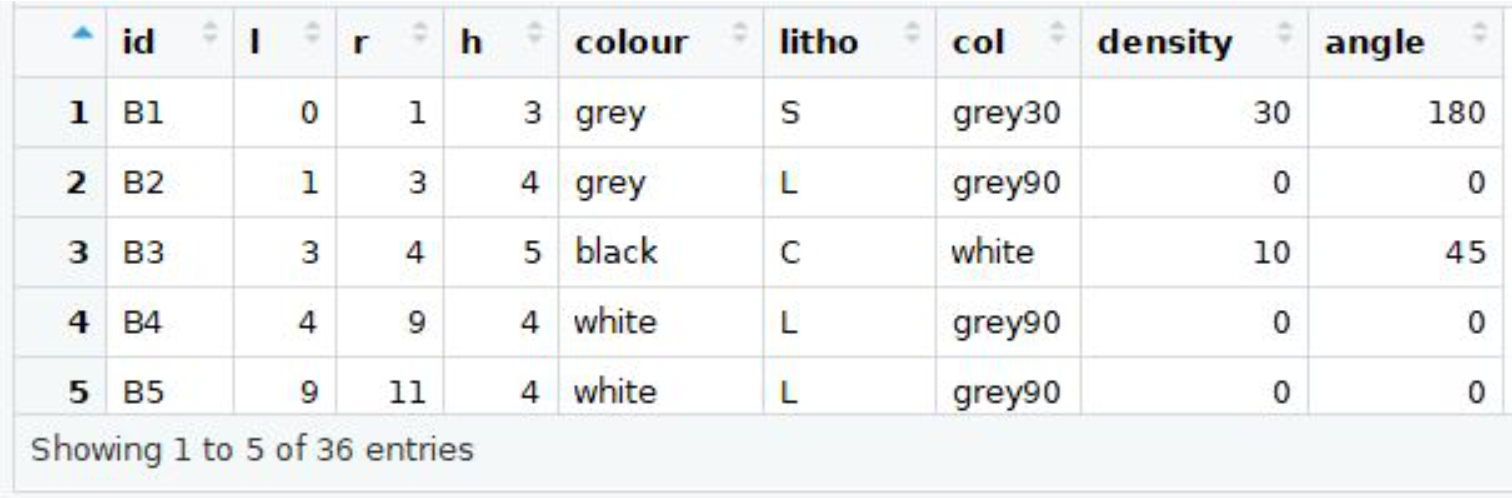
\includegraphics[width=120mm]{Bed legend}
\end{figure}

\begin{example}
plot.new()
plot.window(xlim = c(0,6), ylim = c(-1,77))
minorAxis(2, at.maj = seq(0, 75, 5), n = 5)

# Plotting of the polygons making the litholog, 
# with corresponding symbology:
multigons(basic.log$i, x = basic.log$xy, y = basic.log$dt,
          col = bed.legend$col,
          density = bed.legend$density,
          angle = bed.legend$angle)

# Writing the name of beds, only in beds thick enough
bedtext(labels = bed.example$id, l = bed.example$l, r = bed.example$r,
        x = 0.5,  # x position where to center the text
        ymin = 3) # text is not added in beds thinner than ymin
\end{example}

\begin{figure}[H]
	\centering
	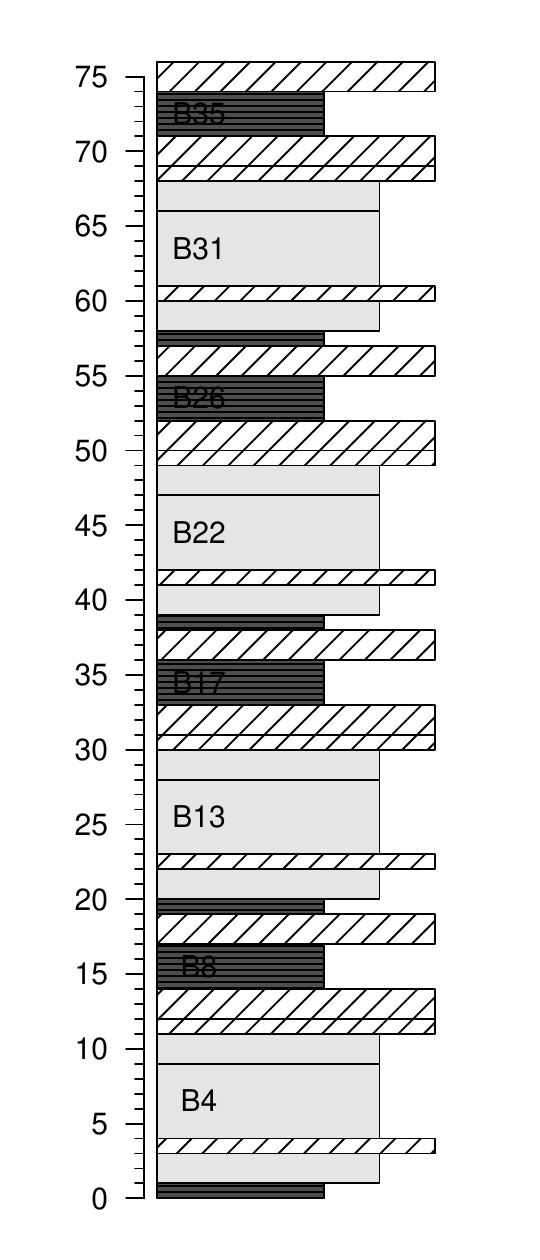
\includegraphics[width=60mm]{base.log}
\end{figure}

To add more complicated beds, the user can add SVG drawings instead of drawing the rectangles through \code{multigons()}, as shown earlier. This is, however, a time-consuming procedure as each bed has to be imported separately. The \code{weldlog()} function can be used to automate the personalization of bed boundaries. It needs to be provided as a polyline, either from R itself (e.g., a sinusoid) or from an SVG file.

\begin{example}
# Code repeated from earlier examples ----
basic.log <- litholog(l = bed.example$l, r = bed.example$r,
                      h = bed.example$h, i = bed.example$id)
legend <- data.frame(litho = c("S", "L", "C"), density = c(30, 0,10),
                     col = c("grey30", "grey90", "white"),
                     angle = c(180, 0, 45), stringsAsFactors = FALSE)
bed.legend <- dplyr::left_join(bed.example,legend, by = "litho")
# ----

# Generation of the boundaries, either sinusoidal or from drawings ---	
s1 <- sinpoint(5,0,0.5,nwave = 1.5)
s2 <- sinpoint(5,0,1,nwave = 3, phase = 0)
s3 <- framesvg(example.liquefaction, 1, 4, 0, 2, plot = FALSE, output = TRUE)

# Visualizing the s3 boundary, i.e., the liquefaction sedimentary feature ----
plot(s3$x, s3$y, cex.axis = 1.2, lwd = 2,
     type = "l", ylab = "", xlab = "", bty = "n", las = 1)
\end{example}

\begin{figure}[H]
	\centering
	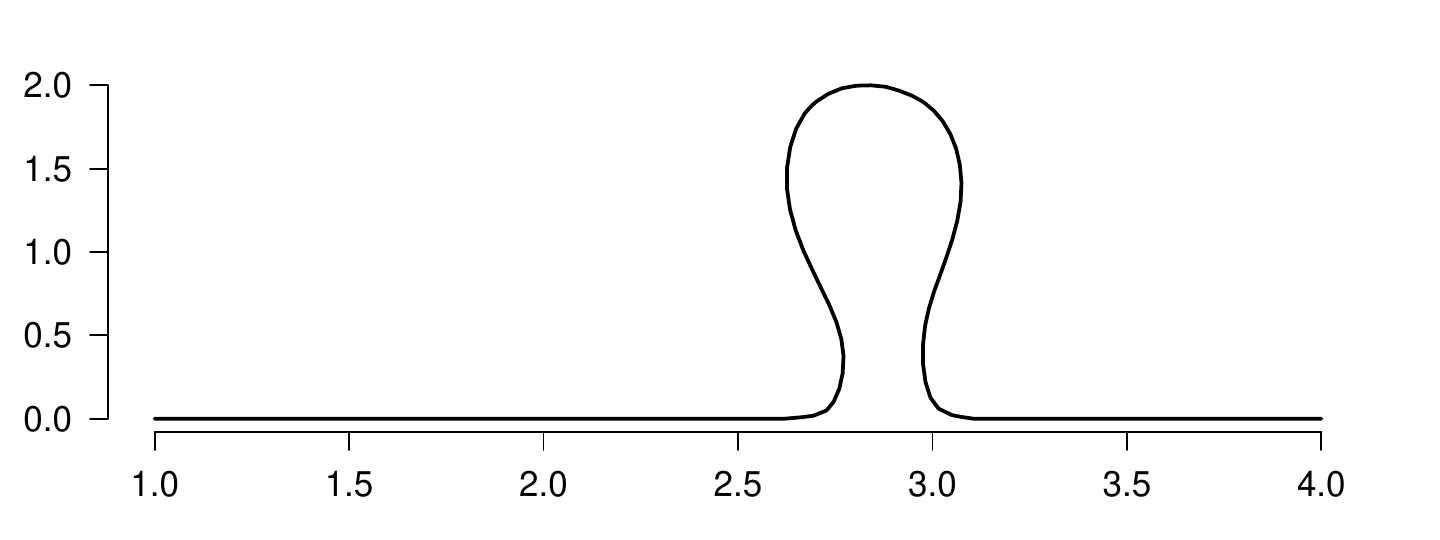
\includegraphics[width=95mm]{liquefaction}
\end{figure}

\begin{example}
# Welding the boundaries to the basic litholog ----
final.log <- weldlog(log = basic.log,
                     dt = boundary.example$dt, # Position of the boundaries 
                                               # to be changed
                     seg = list(s1 = s1, s2 = s2, s3 = s3), # list of segments
                     j = c("s1","s1","s1","s3", # Attributing the segments to 
                           "s2","s2","s1"),     # the respective bed boundaries 
                                                # to  be changed
                     warn = F)

# Visualizing the resulting litholog (similarly to earlier code) ----
plot.new()
plot.window(xlim = c(0,6), ylim = c(-1,77))
minorAxis(2, at.maj = seq(0, 75, 5), n = 5, las = 1)

multigons(final.log$i, x = final.log$xy, y = final.log$dt,
          col = bed.legend$col,
          density = bed.legend$density,
          angle = bed.legend$angle)

bedtext(labels = bed.example$id, l = bed.example$l, r = bed.example$r,
        x = 0.75, ymin = 3)
\end{example}

\begin{figure}[H]
	\centering
	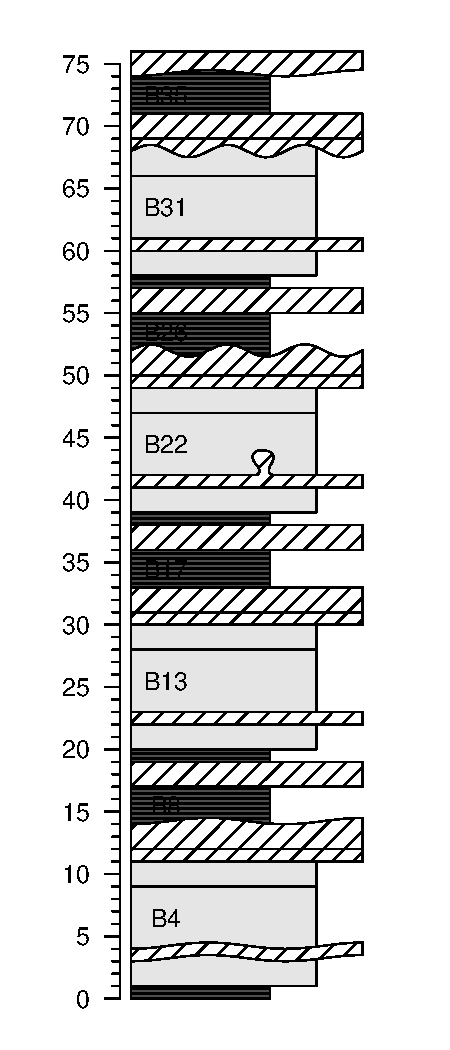
\includegraphics[width=60mm]{boundary.log}
\end{figure}

We see that the thickness of beds can vary. Therefore, a bed boundary can actually vary within a given interval. This raises the question of how to document the position of the bed boundaries in data tables that would only have 2 values for the boundaries (lower and upper) rather than 4 (upper and lower interval of variation for the lower boundary, and upper and lower interval of variation for the upper boundary) or even more (detailing the exact form of the boundaries). We propose a convention for the data tables to be used for the generation of lithologs: the positions of the bed boundaries that are defined in the quantified data have to match in a litholog with the positions of the boundaries of the beds on the axis side of the litholog (usually the left side for single logs). The axis side of the litholog is ideal: it follows a straight vertical line, by an implicit convention followed by the large majority of geologists.

Extra stratigraphic or lithological information, such as geomagnetic chrons, rock color, etc., can be added using the \code{infobar()} function. Any information that can be conveyed by text, such as the positions of samples, can be added using the \code{axis()} or \code{text()} functions.

\begin{example}
# Code repeated from earlier examples ----
basic.log <- litholog(l = bed.example$l, r = bed.example$r,
                      h = bed.example$h, i = bed.example$id)
legend <- data.frame(litho = c("S", "L", "C"), density = c(30, 0,10),
                     col = c("grey30", "grey90", "white"),
                     angle = c(180, 0, 45), stringsAsFactors = FALSE)
bed.legend <- dplyr::left_join(bed.example,legend, by = "litho")
s1 <- sinpoint(5,0,0.5,nwave = 1.5)
s2 <- sinpoint(5,0,1,nwave = 3, phase = 0)
s3 <- framesvg(example.liquefaction, 1, 4, 0, 2, plot = FALSE, output = TRUE)
final.log <- weldlog(log = basic.log, dt = boundary.example$dt,
                     seg = list(s1 = s1, s2 = s2, s3 = s3),
                     j = c("s1","s1","s1","s3","s2","s2","s1"), warn = F)
\end{example}
\newpage
\begin{example}
# Visualizing the resulting litholog (similarly to earlier code) ----
plot.new()
plot.window(xlim = c(-1.5,8), ylim = c(-1,81))
minorAxis(2, at.maj = seq(0, 75, 5), n = 5, las = 1)

multigons(final.log$i, x = final.log$xy, y = final.log$dt,
          col = bed.legend$col,
          density = bed.legend$density,
          angle = bed.legend$angle)

bedtext(labels = bed.example$id, l = bed.example$l, r = bed.example$r,
        x = 0.5, ymin = 2)

# Making a data table for the symbology of magnetochrons
legend.chron <- data.frame(polarity = c("N", "R"),
                           bg.col = c("black", "white"),
                           text.col = c("white", "black"),
                           stringsAsFactors = FALSE)

# Merging symbology with a data table of chrons
chron.legend <- dplyr::left_join(chron.example, legend.chron, by = "polarity")

# Plotting the chrons with the given symbology
infobar(-1.5, -1, chron.legend$l, chron.legend$r,
        labels = chron.legend$polarity,
        m = list(col = chron.legend$bg.col),
        t = list(col = chron.legend$text.col),
        srt = 0)

# Adding color information
colour <- bed.example$colour
colour[colour == "darkgrey"] <- "grey20"
colour[colour == "brown"]    <- "tan4"

# Plotting the color next to the litholog
infobar(-0.25, -0.75, bed.example$l, bed.example$r, 
        m = list(col = colour))

text(-0.5, 79, "Colour", srt = 90)
text(-1.25, 79, "Magnetochrons", srt = 90)

axis(4, at = proxy.example$dt, labels = proxy.example$name, 
     pos = 6, lwd = 0, lwd.ticks = 1, las = 1)	
\end{example}

\begin{figure}[H]
	\centering
	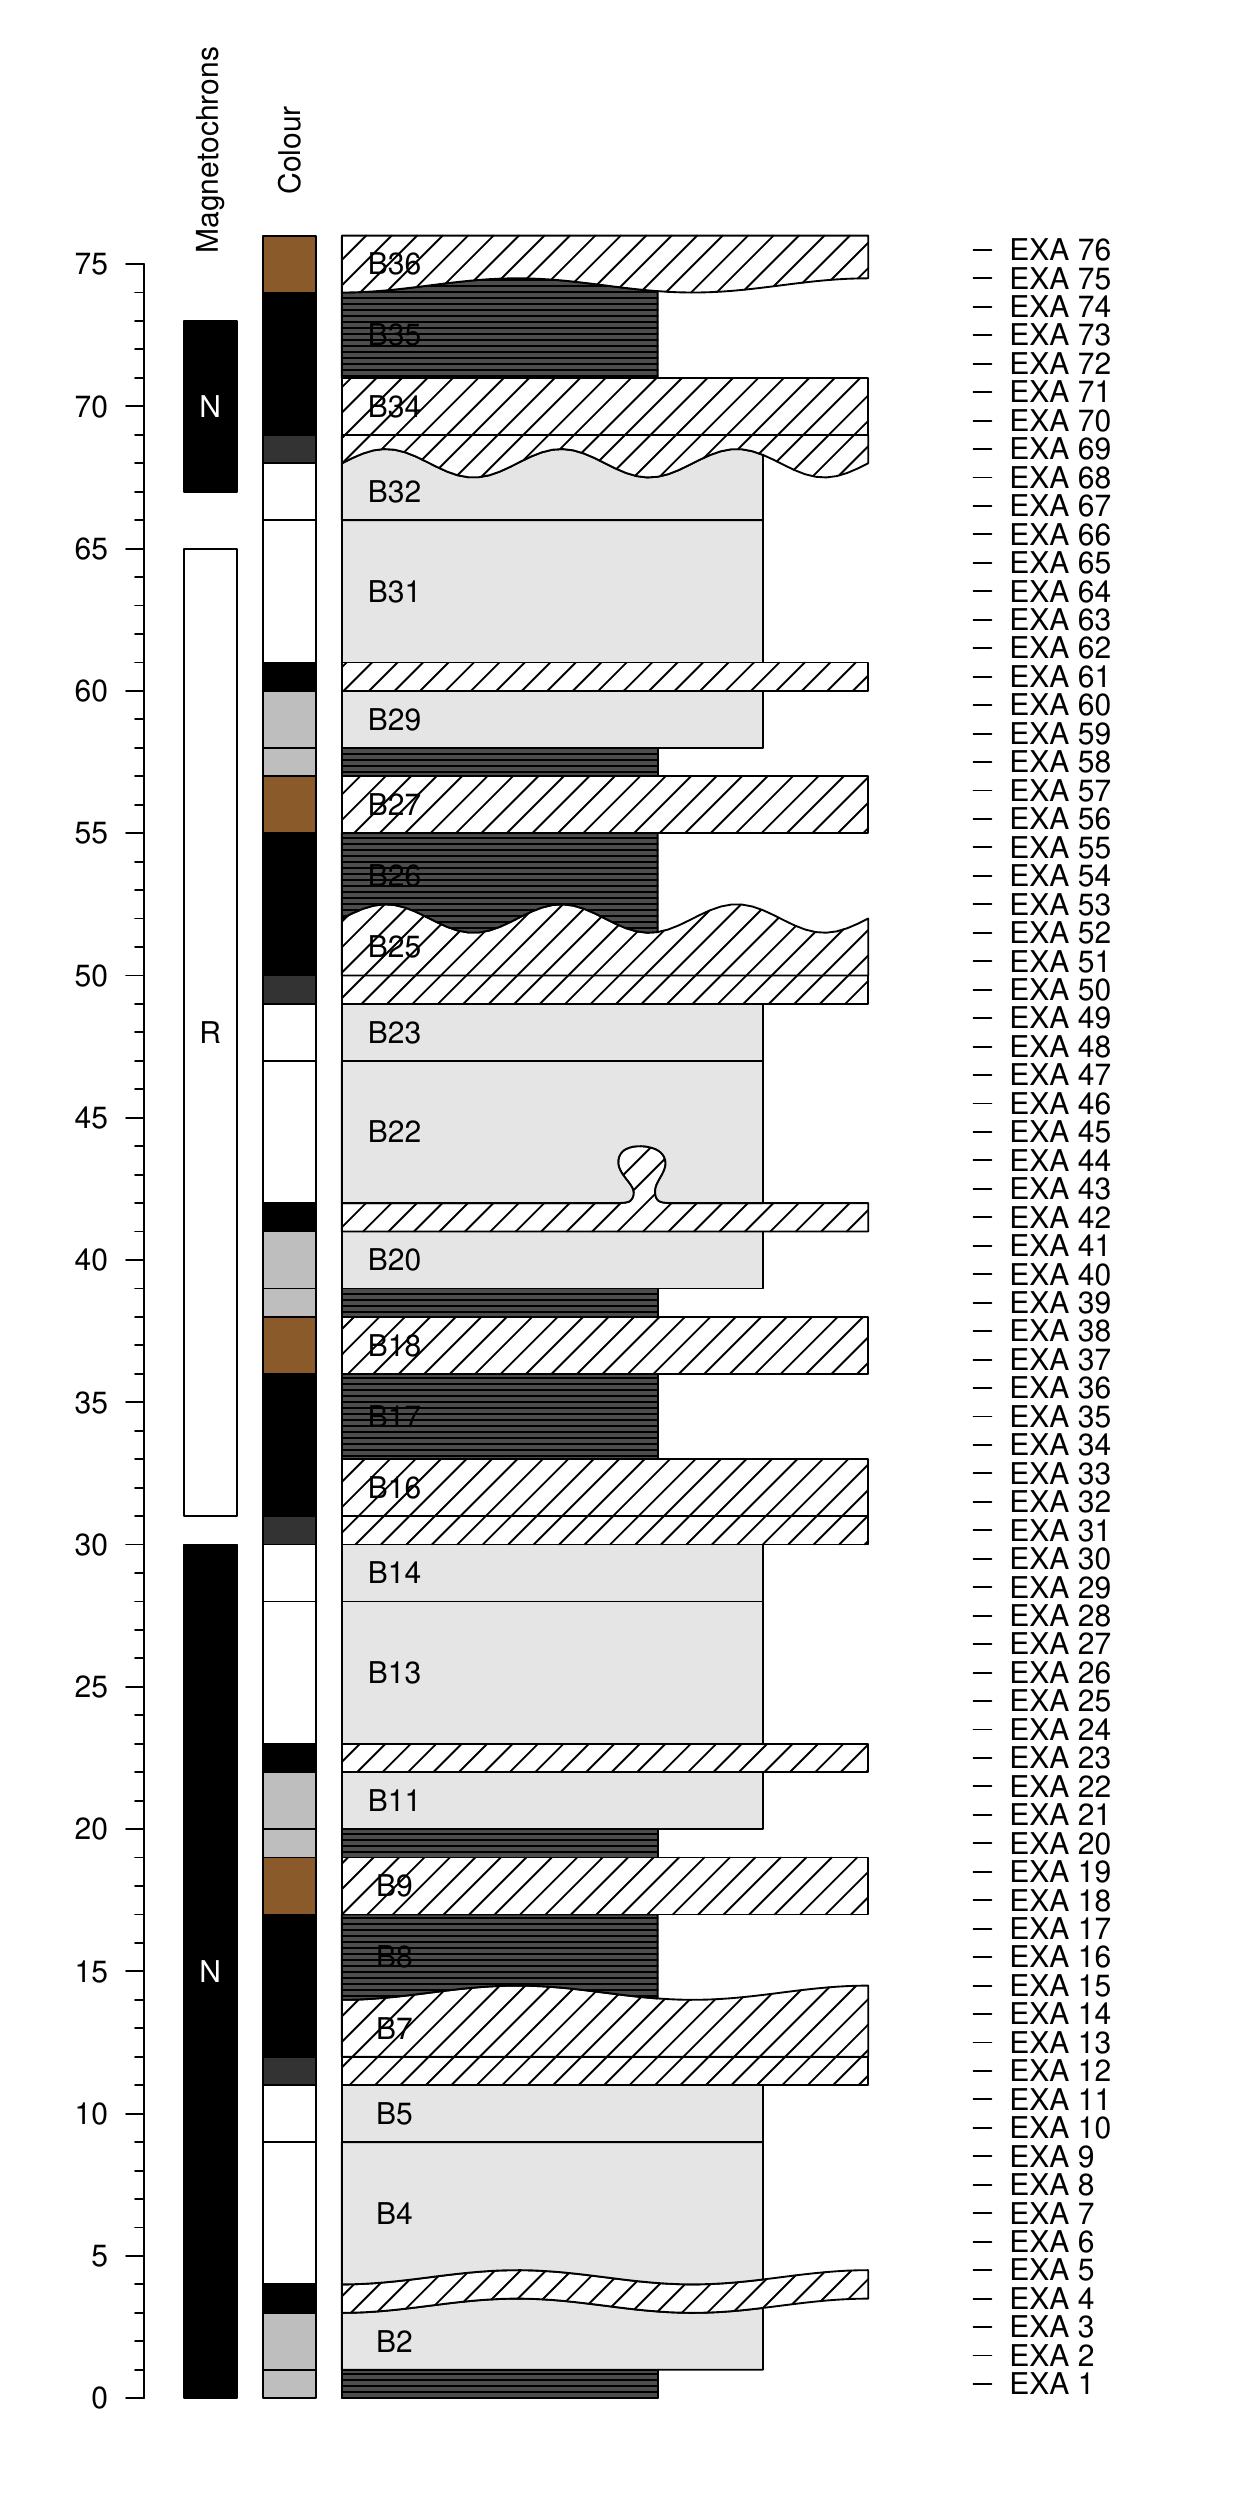
\includegraphics[width=97mm]{advanced.log}
\end{figure}

Other plots can be drawn along the litholog. Great care should be taken to ensure that the depth axis is identical in all plots. To ensure that, two components have to be taken into account: the \code{ylim} argument of \code{plot.window()} or \code{plot()} (for vertical logs, otherwise the \code{xlim} argument), and the graphical parameters defined by the \code{par()} function, especially the \code{yaxs} (for vertical logs, otherwise \code{xaxs}) and the \code{mar} arguments. The \code{ylim} argument controls the range of the axis, but the exact range will depend on the \code{yaxs} argument. Indeed, the default setting of \code{yaxs} is \code{"r"}, which stands for regular, and means that the data range defined by \code{ylim} is extended by 4 percent at each end. Such extension can be unwanted in very long lithologs. Alternatively, the \code{yaxs} argument can be set as \code{"i"}, which stands for 'internal', and prevents the extension of the range defined by \code{ylim}. The \code{mar} argument controls the margin size of the plotting zone. To add plots along the litholog, a simple way is to use the \code{mfrow} argument in the \code{par()} function to define several plotting areas, which will be used by the successively called plots.

\begin{example}
# Code repeated from earlier examples ----
basic.log <- litholog(l = bed.example$l, r = bed.example$r,
                      h = bed.example$h, i = bed.example$id)
legend <- data.frame(litho = c("S", "L", "C"),
                     col = c("grey30", "grey90", "white"),
                     density = c(30, 0,10),
                     angle = c(180, 0, 45), stringsAsFactors = FALSE)
bed.legend <- dplyr::left_join(bed.example,legend, by = "litho")
s1 <- sinpoint(5,0,0.5,nwave = 1.5)
s2 <- sinpoint(5,0,1,nwave = 3, phase = 0)
s3 <- framesvg(example.liquefaction, 1, 4, 0, 2, plot = FALSE, output = TRUE)
final.log <- weldlog(log = basic.log, dt = boundary.example$dt,
                     seg = list(s1 = s1, s2 = s2, s3 = s3),
                     j = c("s1","s1","s1","s3","s2","s2","s1"), warn = F)
# ----

opar <- par() # Save initial graphical parameters (IGP)
par(mfrow = c(1,2),  # Set two vertical plots along each other
    yaxs = "r",                  # Default setting, adds 4% more range for y 
    mar = c(5.1, 4.1, 4.1, 0.1)) # Change settings for margins

# Visualizing the resulting litholog (similarly to earlier code) ----
plot.new()
plot.window(xlim = c(0,6), ylim = c(-1,77))
minorAxis(2, at.maj = seq(0, 75, 5), n = 5, las = 1)

multigons(final.log$i, x = final.log$xy, y = final.log$dt,
          col = bed.legend$col,
          density = bed.legend$density,
          angle = bed.legend$angle)

bedtext(labels = bed.example$id, l = bed.example$l, r = bed.example$r,
        x = 0.75, ymin = 3)

# Visualizing quantified values along the litholog ----

par(mar = c(5.1, 0.1, 4.1, 4.1)) # Change settings for margins of 2nd plot

plot.new()
plot.window(xlim = c(-2*10^-8,8*10^-8), ylim = c(-1,77)) # ylim similar to
                                                         # litholog
                                                         
minorAxis(4, at.maj = seq(0, 75, 5), n = 5, las = 1) # Repetition of the axis to
                                                     # check both sides are matching

lines(proxy.example$ms, proxy.example$dt, type = "o", pch = 19)
axis(1)
title(xlab = "Magnetic Susceptibility")	

par(mar = opar$mar, mfrow = opar$mfrow, yaxs = opar$yaxs) # Restore IGP
\end{example}

\begin{figure}[H]
	\centering
	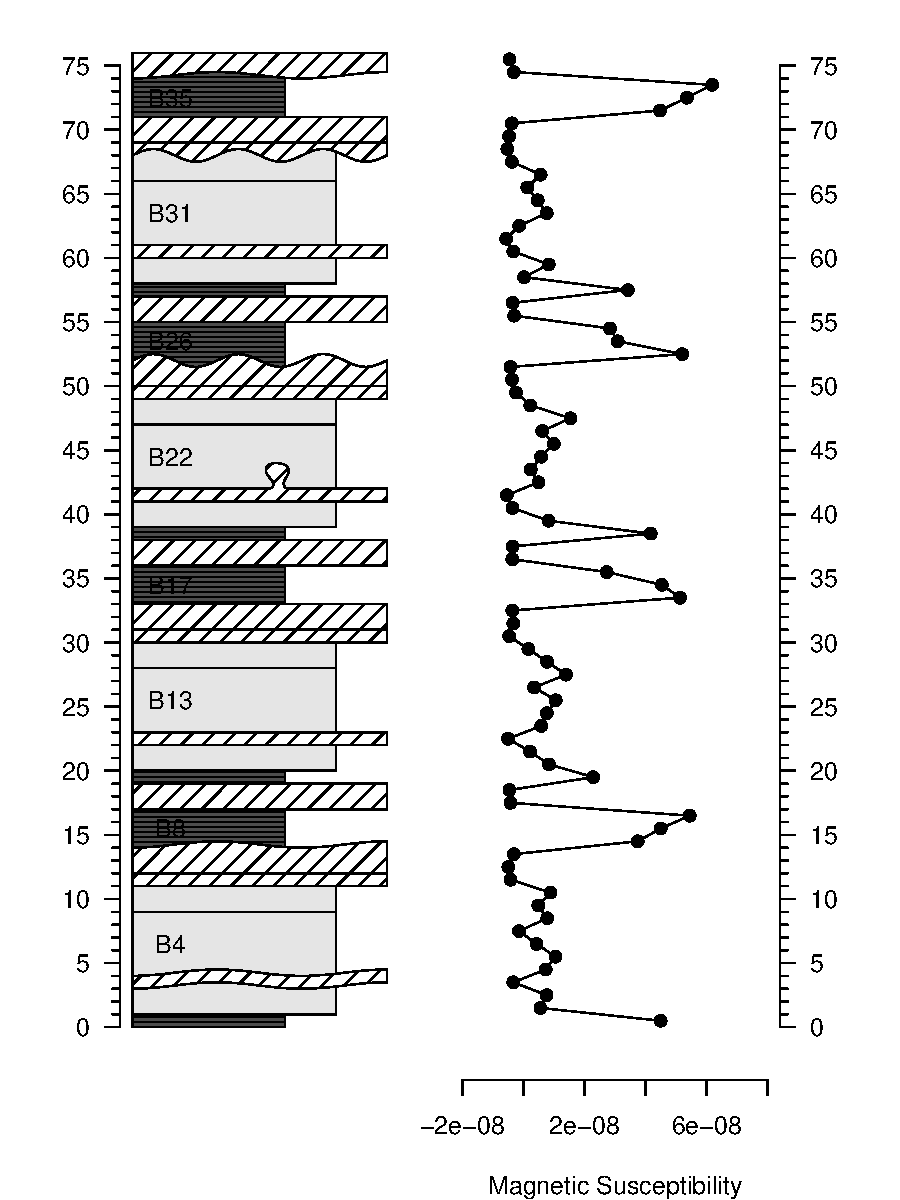
\includegraphics[width=77mm]{proxy.log}
\end{figure}

A legend plot can be generated using the \code{nlegend()} function. The basic idea is to make a subplot for each symbol (using the \code{par()} function, for instance), in which the \code{nlegend()} function calls a new plot leaving free space for the symbol (included in [-1, 1], both for x and y coordinates), and adds the text description. This scheme improves automation, e.g., by simplifying the symbol generation of rock types in a function as shown in the code below:

\begin{example}
legend <- data.frame(litho = c("S", "L", "C"),             # Symbology 
                     col = c("grey30", "grey90", "white"), # data table
                     density = c(30, 0,10), angle = c(180, 0, 45),
                     stringsAsFactors = FALSE)

f <- function(legend_row) # To simplify coding, we design here a function 
                          # plotting rectangles with the desired symbology
{
   multigons(i = rep(1, 4), c(-1,-1,1,1), c(-1,1,1,-1),
             col = legend$col[legend_row], 
             density = legend$density[legend_row],
             angle = legend$angle[legend_row])
}	

opar <- par() # Save initial graphical parameters
par(mar = c(0,0,0,0), mfrow = c(5,1)) # Make 5 plot windows

nlegend(t = "Shale", cex = 2) # The cex parameter controls the size of the text
f(1) # 1 stands for the first row of the symbology data table
nlegend(t = "Limestone", cex = 2)
f(2)
nlegend(t = "Chert", cex = 2)
f(3)

nlegend(t = "Ammonite", cex = 2)
centresvg(example.ammonite, 0,0,xfac = 0.5)
nlegend(t = "Belemnite", cex = 2)
centresvg(example.belemnite, 0,0,xfac = 0.5)

par(mar = opar$mar, mfrow = opar$mfrow) # Restore initial graphical parameters
\end{example}

\begin{figure}[H]
	\centering
	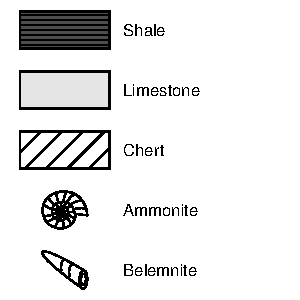
\includegraphics[width=60mm]{legend.log}
\end{figure}

As lithologs can be longer than a single printable page, it is sometimes necessary to split them into separate plots to be displayed on successive pages of a text document. This can be done by grouping all the drawing functions used to generate the litholog into a single function, with \code{ylim} as an argument. This function can be iterated with successive \code{ylim} intervals.

Functions that generate several plots will generate the corresponding pages in the PDF generated by \code{pdfDisplay()}. All the pages have to be of the same dimensions. To integrate these successive litholog figures into a larger document that would include all the litholog parts, the associated legend, a text description of the section, etc., \href{https://www.latex-project.org/}{LaTeX} can be used. A \textbackslash foreach loop in LaTeX can then be applied to import all the pages using the \textbackslash includegraphics function.

\begin{example}
# Code repeated from earlier examples ----
basic.log <- litholog(l = bed.example$l, r = bed.example$r,
                      h = bed.example$h, i = bed.example$id)
legend <- data.frame(litho = c("S", "L", "C"),
                     col = c("grey30", "grey90", "white"),
                     density = c(30, 0,10),
                     angle = c(180, 0, 45), stringsAsFactors = FALSE)
bed.legend <- dplyr::left_join(bed.example,legend, by = "litho")
s1 <- sinpoint(5,0,0.5,nwave = 1.5)
s2 <- sinpoint(5,0,1,nwave = 3, phase = 0)
s3 <- framesvg(example.liquefaction, 1, 4, 0, 2, plot = FALSE, output = TRUE)
final.log <- weldlog(log = basic.log, dt = boundary.example$dt,
                     seg = list(s1 = s1, s2 = s2, s3 = s3),
                     j = c("s1","s1","s1","s3","s2","s2","s1"), warn = F)
legend.chron <- data.frame(polarity = c("N", "R"),
                           bg.col = c("black", "white"),
                           text.col = c("white", "black"),
                           stringsAsFactors = FALSE)
chron.legend <- dplyr::left_join(chron.example,legend.chron, by = "polarity")
colour <- bed.example$colour
colour[colour == "darkgrey"] <- "grey20"
colour[colour == "brown"]    <- "tan4"
# ----

# Function that will draw a litholog, with personalized coordinates control
log.function <- function(xlim = c(-2.5,7), ylim = c(-1,77))
{
   plot.new()
   plot.window(xlim = xlim, ylim = ylim)
   minorAxis(2, at.maj = seq(0, 75, 5), n = 5, pos = -1.75, las = 1)
	
   multigons(final.log$i, x = final.log$xy, y = final.log$dt,
             col = bed.legend$col,
             density = bed.legend$density,
             angle = bed.legend$angle)
	
	
   bedtext(labels = bed.example$id, l = bed.example$l, r = bed.example$r,
           x = 1, edge = TRUE, ymin = 2)
	
   centresvg(example.ammonite, 6,
             fossil.example$dt[fossil.example$type == "ammonite"],
             xfac = 0.5)
   centresvg(example.belemnite, 6,
             fossil.example$dt[fossil.example$type == "belemnite"],
             xfac = 0.5)
	
   infobar(-1.5, -1, chron.legend$l, chron.legend$r,
           labels = chron.legend$id, m = list(col = chron.legend$bg.col),
           t = list(col = chron.legend$text.col))
   infobar(-0.25, -0.75, bed.example$l, bed.example$r, 
           m = list(col = colour))
}

# In this gr() function, log.function() is repeated, which plots the
# desired parts of the litholog

gr <- function()
{
   opar <- par()  # Save initial graphical parameters
   par(mar = c(1,2,1,2), yaxs = "i")
   ylim <- c(0,40) # Initial range to be plotted
   
   for(i in 1:0) log.function(ylim = ylim + 40*i) # Iteration of the plotting
   # The drawing range's length is iteratively added to the range already drawn

   par(mar = opar$mar, yaxs = opar$yaxs) # Restore initial graphical parameters
}

# Integration of gr() in pdfDisplay to make PDFs
pdfDisplay(gr(), name = "divided log", width = 3, height = 5)	
\end{example}

\begin{figure}[H]
	\centering
	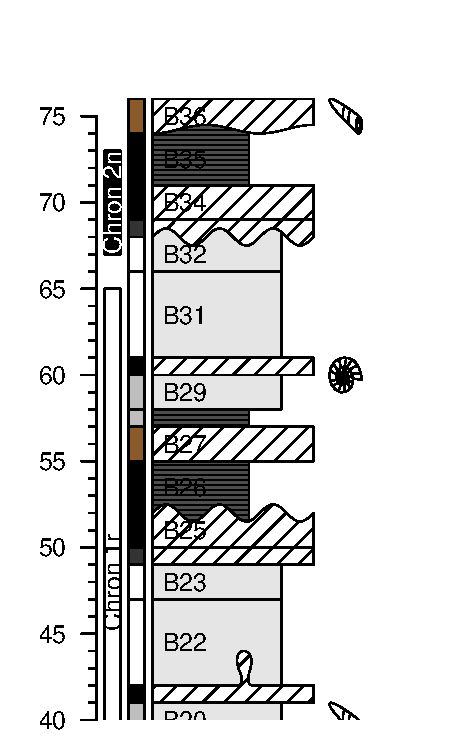
\includegraphics[width=60mm, page=1]{divided log}
\end{figure}

\begin{figure}[H]
	\centering
	\includegraphics[width=60mm, page=2]{divided log}
\end{figure}

\begin{example}
# The code can be adapted to divide the plot differently, 
# and to add other plots along the litholog
	
gr2 <- function()
{
   opar <- par() # Save initial graphical parameters (IGP)
		
   low  <- c(-5, 25, 55) # Another way of defining the dimensions
   high <- c( 25, 55, 85) # of succesive plotting windows
		
   for(i in 3:1){  # Inverted order to have them in stratigraphic order
			
      par(mfrow = c(1,2), yaxs = "i") # Plot in two columns, same yaxs for both
      par(mar = c(5,2,1,0)) # Define margins for first plot (left)
			
      log.function(ylim = c(low[i], high[i]))
			
      par(mar = c(5,0,1,1)) # Second plot (right): change only the vertical  
                            # margins (2nd and 4th)
			
      plot.new()
      plot.window(xlim = c(-2*10^-8,8*10^-8), ylim = c(low[i], high[i]))
      lines(proxy.example$ms, proxy.example$dt, type = "o", pch = 19)
      axis(1)
      title(xlab = "Magnetic Susceptibility")
			
   }
		
    par(mar = opar$mar, yaxs = opar$yaxs, mfrow = opar$mfrow) # Restore IGP
}
	
pdfDisplay(gr2(), name = "divide in 3", wi = 5, he = 7)
\end{example}

\begin{figure}[H]
	\centering
	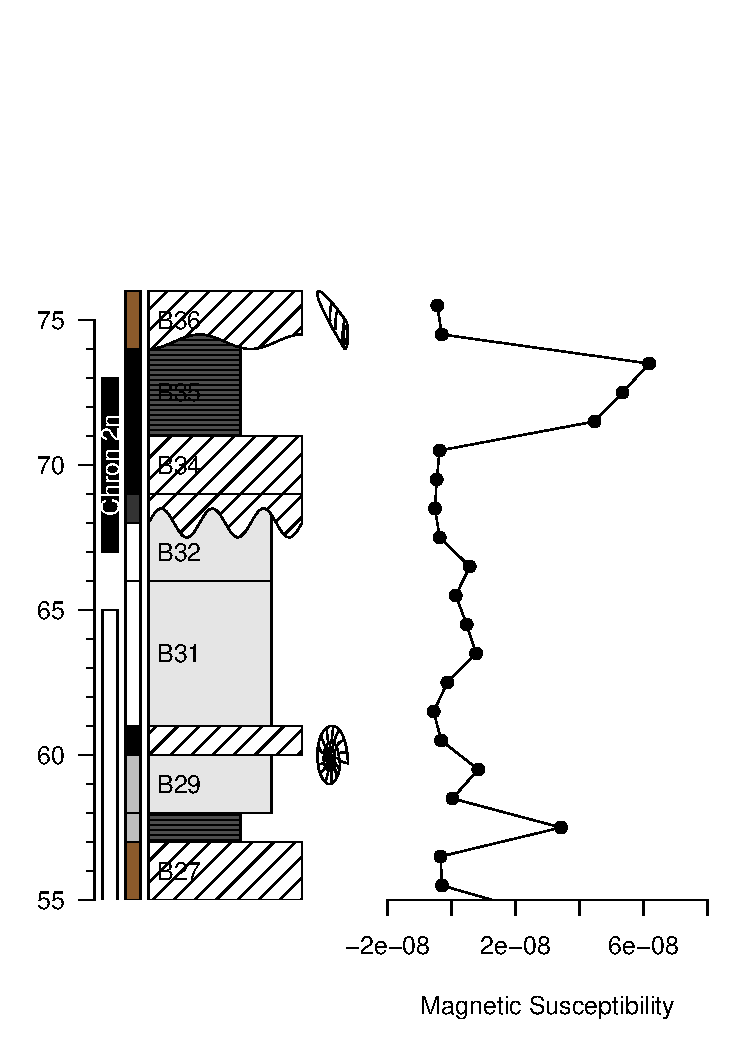
\includegraphics[width=85mm, page=1]{divided2}
\end{figure}

\begin{figure}[H]
	\centering
	\includegraphics[width=85mm, page=2]{divided2}
\end{figure}

\begin{figure}[H]
	\centering
	\includegraphics[width=85mm, page=3]{divided2}
\end{figure}

The preceding examples illustrate some of the capabilities of the \textbf{StratigrapheR} package. However, an important question remains unanswered: have we overcome the "from art to useful data" challenge? We will illustrate our answer by importing the computer-drawn litholog from Fig.~\ref{figure:drawnlog}. We will also take the opportunity to show how \textbf{StratigrapheR} can help in the comparison and correlation of sections. For that purpose, we plot two lithologs in front of each other and visually link them using the \code{ylink()} function. \code{ylink()} currently only works in single window plots, i.e., having a coherent x and y coordinate system. Therefore, we need to change the coordinate system of one of the two lithologs.

Prior to importing it into R using \code{pointsvg()}, all the lines and polygons in the litholog in Fig.~\ref{figure:drawnlog} are sparsely interpolated, and all the curves are converted into straight lines. To have perfect positioning in x and y coordinates, the initial drawing is surrounded by a rectangle having known coordinates. Afterward, the figure is saved as an SVG file. All this takes less than a minute with vector graphics software (here using CorelDRAW). The sparse interpolation means that the figures will be angular (take, for instance, the initially elliptical lens containing brachiopods at 34.5 m, when imported by the code here below, it becomes clearly polygonal). If smoother curves are desired, the amount of interpolated points can be increased. When the figure is imported by \code{pointsvg()}, the rectangle defines the borders of the figure, which by default are set at [-1, 1] in x and y. These coordinates are changed using \code{framesvg()} by providing the initial coordinates of the rectangle as \code{xmin}, \code{xmax}, \code{ymin}, and \code{ymax}. Having served its purpose as a reference in x and y, the rectangle can be removed directly in \code{framesvg()} using the \code{forget} argument.

\begin{example}
svg.file.directory <- tempfile(fileext = ".svg")   # Creates temporary file
writeLines(example.HB2000.svg, svg.file.directory) # Writes svg in the file

# Log: 1 Humblet and Boulvain 2000 ----

a   <- pointsvg(svg.file.directory) # Import the svg
out <- framesvg(a, 
                xmin = 0, xmax = 5,    # Initial coordinates of the 
                ymin = 27, ymax = 36,  # rectangle (see SVG file)
                output = T,  # This allows to output the changed coordinates
                forget = "P287")  # 'forget' removes the rectangle added in the
                                  # svg to serve as a referential in x and y
                                
# Log 2: Code repeated from earlier examples ----

basic.log <- litholog(l = bed.example$l, r = bed.example$r,
                      h = bed.example$h, i = bed.example$id)
legend <- data.frame(litho = c("S", "L", "C"),
                     col = c("grey30", "grey90", "white"),
                     density = c(30, 0,10),
                     angle = c(180, 0, 45), stringsAsFactors = FALSE)
bed.legend <- dplyr::left_join(bed.example,legend, by = "litho")
s1 <- sinpoint(5,0,0.5,nwave = 1.5)
s2 <- sinpoint(5,0,1,nwave = 3, phase = 0)
s3 <- framesvg(example.liquefaction, 1, 4, 0, 2, plot = FALSE, output = TRUE)
final.log <- weldlog(log = basic.log, dt = boundary.example$dt,
                     seg = list(s1 = s1, s2 = s2, s3 = s3),
                     j = c("s1","s1","s1","s3","s2","s2","s1"), warn = F)

# Plotting two logs in front of each other ----

plot.out   <- out # Save a version of the svg object
tie.points <- data.frame(l = c(20,35,54,66),            # Define points to correlate
                         r.raw = c(29.8,31,32.5,33.25)) # the two sections in  
                                                        # their own depth scales

plot.out$x   <- 15 - out$x                   # Change the coordinates for
plot.out$y   <- 10*(out$y - 27.5)            # second litholog (imported 
axs2         <- 10*(28:35 - 27.5)            # from Fig. 1), to plot it t
tie.points$r <- 10*(tie.points$r.raw - 27.5) # in front of the first litholog

g <- function()
{
   opar <- par()  # Save initial graphical parameters
   par(mar = c(1,4,1,4))
   plot.new()
   plot.window(xlim = c(0,15), ylim = c(0,75))
   minorAxis(2, at.maj = seq(0,75, 5), n = 5, las = 1, cex.axis = 1.2)
   minorAxis(4, at.maj = axs2, labels = 28:35, n = 10, las = 1, cex.axis = 1.2)
	
   multigons(final.log$i, x = final.log$xy, y = final.log$dt,
             col = bed.legend$col,
             density = bed.legend$density,
             angle = bed.legend$angle)
	
   placesvg(plot.out, col = "white") # Adding the drawn plot
	
   ylink(tie.points$l, tie.points$r, 6, 9, ratio = 0.5,  # Correlation between 
         l = list(lty = c(1,2,2,1), lwd = 2))            # the two plots
	      
   par(mar = opar$mar) # Restore initial graphical parameters
		
}

pdfDisplay(g(), "Log Correlation")
\end{example}

\begin{figure}[H]
	\centering
	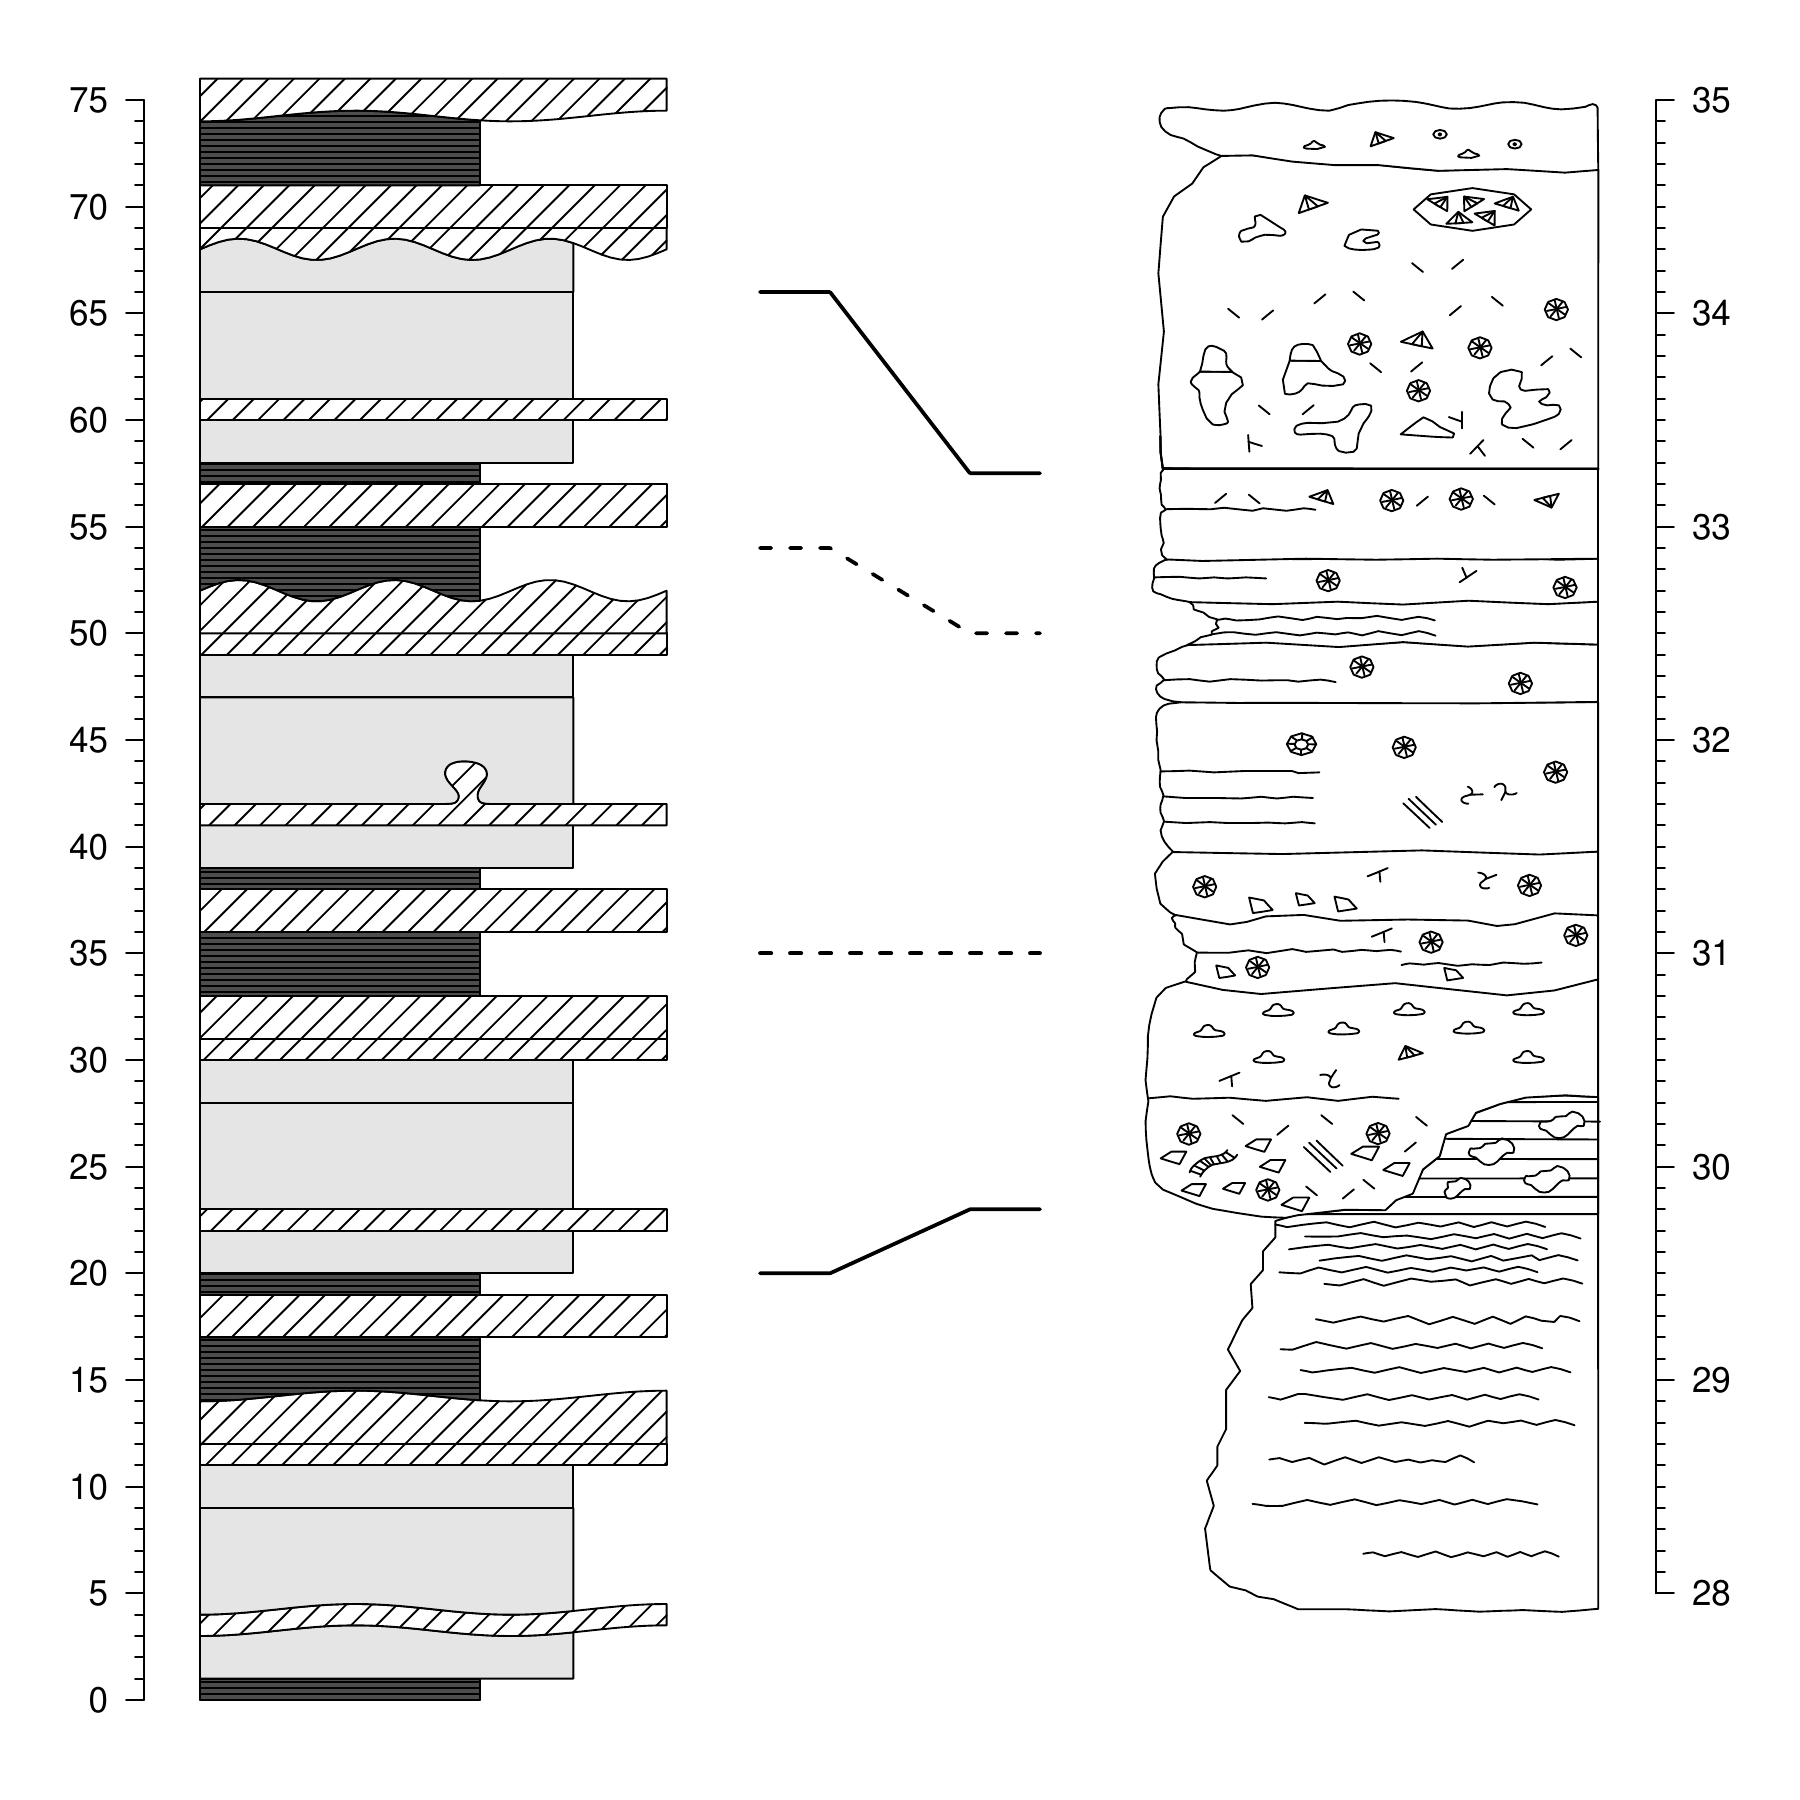
\includegraphics[width=105mm]{Log Correlation}
\end{figure}

 The most obvious discrepancy between the original computer-drawn version (Fig.~\ref{figure:drawnlog}) and the one imported in R is the lack of color in the latter. We could have identified all the gray polygons one by one and provided them with a color symbology, but such a tedious task would go against the motto of simplifying data management. This highlights that at the moment, the conversion of lithologs "from art to useful data" is not as straightforward as it could be, yet it is not too far out of our reach. 

\section{New R functions for geological and general purpose}

\textbf{StratigrapheR} was designed in a modular way: low-level general-purpose functions were implemented to simplify the development of higher-level functions. The package also hosts a couple of functions that are not specifically related to lithologs but could be of great use, especially to geologists, and to other developers. We present a few of these functions in this chapter to promote the use of modular and general-purpose functions and to help other developers making their own functions.

\begin{itemize}
	\item \code{divisor()}: finds the greatest common rational divisor (GCRD) of a set of values, typically depth, height, or time in time series. This function is important as it allows to transform floating-point values into integers (within the precision range allowed by floating-point arithmetic) by dividing them by the GCRD. We highlight its high potential to automate data processing, especially to interpolate the irregularly-sampled depth, height, or time values that are omnipresent in geology (interpolation by the GCRD preserves the original values). This function is somewhat empirical and would benefit from improvements (among others to reduce the computing time, typically in the case where the GCRD is significantly smaller than the input values), but this would require expertise in mathematics and informatics that the authors do not have. We hope that open-source developers will respond to this challenge. 
	\item \code{every\_nth()}: leaves or removes values at position indexes of multiples of a given amount (n). This is typically useful to discriminate major and minor ticks of a personalized axis.
	\item \code{in.window()}: this function can serve as a base for windowing (typically to perform a moving average). It gives a matrix of all the points included in each successive window (in depth, height, or time). We illustrate this with irregularly sampled data points.
	
\begin{example}
window <- in.window(irreg.example$dt,  # Depth values
                    w = 30,   # Size of the window
                    xout = seq(0, 600, 20),  # Center position of windows
                    xy = irreg.example$xy)  # Intensity values (or other)
		
mov.mean <- rowMeans(window$xy, na.rm = TRUE) # Average of the intensity 
                                              # values in windows
		
presence <- matrix(as.integer(!is.na(window$xy)), # Discriminate between NA 
                   ncol = ncol(window$xy))        # values and intensity values 
amount   <- rowSums(presence)                     # to determine the amount of 
                                                  # real values in each window
                                                  # (example of window calculation)
		                                                  
opar <- par() # Save initial graphical parameters
par(mfrow = c(2,1), mar = c(0,4,0,0))
plot(irreg.example$dt, irreg.example$xy, type = "o", pch = 19,
     xlim = c(0,600), xlab = "dt", ylab = "xy and moving average", axes = F)
lines(window$xout, mov.mean, col = "red", lwd = 2)
axis(2, las = 1)
		 
par(mar = c(5,4,0,0))
plot(window$xout, amount, pch = 19, xlim = c(0,600), ylim = c(0,25), 
     xlab = "dt", ylab = "amount of points in the windows", axes = F)
axis(1)
axis(2, las = 1)
   
par(mar = opar$mar, mfrow = opar$mfrow) # Restore initial graphical parameters  
                                            
\end{example}
	
\begin{figure}[H]
\centering
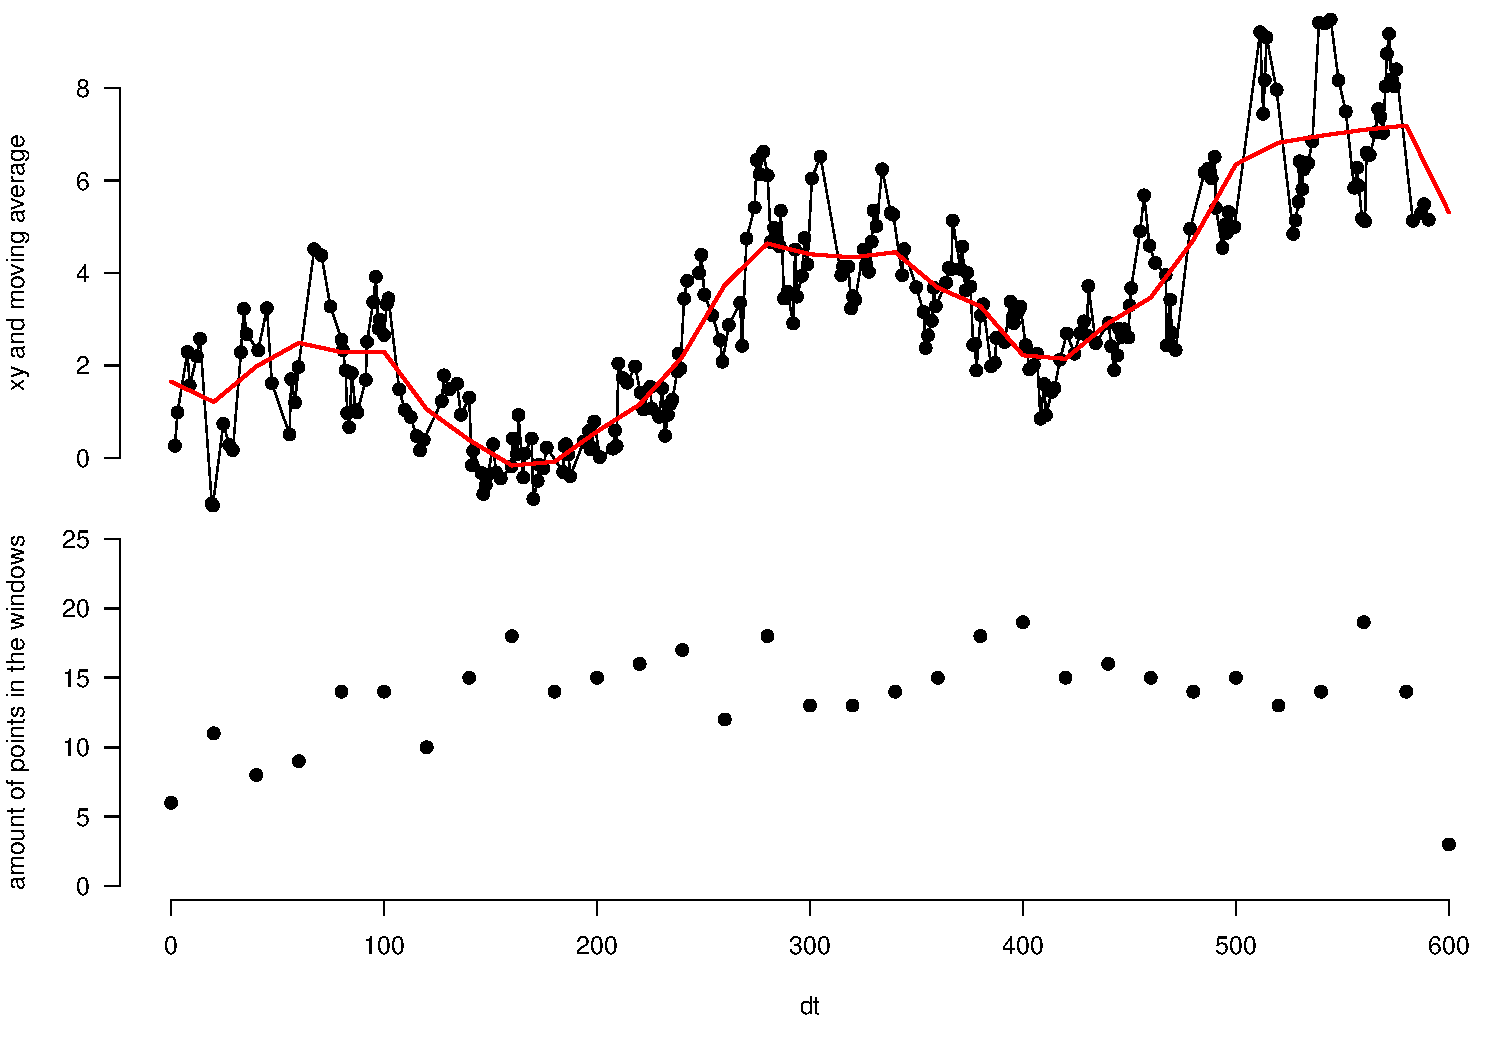
\includegraphics[width=120mm]{MovingAverage}
\end{figure}

	\item \code{nset()}: finds the position of a given amount of values (n) having a common identification code, selecting either the n first or the n last ones, or signaling that they are not available (\code{NA}). This is useful to homogenize replicate measurement values.

\begin{example}
id   <- c("samp1", "samp1", "samp2", "samp3", "samp3", "samp3")
meas <- c(   0.45,    0.55,     5.0,     100,     110,     120)
	
new_sequence <- nset(id, 2, warn = F)
	
new_sequence
#>       [,1] [,2]
#> samp1    1    2
#> samp2    3   NA
#> samp3    4    5
	
clean_meas <- matrix(meas[new_sequence], ncol = 2)
	
row.names(clean_meas) <- unique(id)
	
clean_meas
#>         [,1]   [,2]
#> samp1   0.45   0.55
#> samp2   5.00     NA
#> samp3 100.00 110.00

\end{example}

	\item \code{seq\_mult()}: gives a sequence of numbers that are reordered by a given divisor of the length of the sequence (e.g., \code{seq\_mult(10,5)} gives the sequence 1, 6, 2, 7, 3, 8, 4, 9, 5, 10). This is useful to reorder and manipulate repetitive sequences (e.g., changing 1, 2, 3, 4, 5, 1, 2, 3, 4, 5 into 1, 1, 2, 2, 3, 3, 4, 4, 5, 5 and back). 
\end{itemize}

\section{Present limitations and prospects for the future}

\textbf{StratigrapheR}, for the moment, uses the \strong{base} graphics in R. This is a choice that was made in the initial development phase of the package, as the base graphics (also called traditional graphics) are easy to learn for R beginners and are relatively robust, compared to their alternative; the \strong{grid} graphics \citep{murrell_r_2012}. The grid graphics are the basis for the \CRANpkg{lattice} \citep{sarkar_lattice_2008} and \CRANpkg{ggplot2} \citep{wickham_ggplot2_2016} graphical packages. Grid graphics allow more sophistication than the base graphics, but at the price of a more complicated implementation \citep{murrell_r_2012}. However, grid graphics would make the entire litholog generation process more efficient, especially by using the concept of grob (which stands for GRaphical OBject). Grobs are R objects that save all the information of a plot, which can then be modified without needing to alter or rewrite the code made to generate the grobs. This would avoid any unnecessary repetition of code. Revisiting the examples in the article, you will see that the code needed for litholog generation does require writing the entire plotting functions at each plot generation or inserting them into a function. On the other hand, elements of a plot made in grid graphics can be expressed via grobs and can be reassembled to generate a modified version of the plot without explicitly making a function or repeating the code. This would further simplify drawing different parts of the same plot on several pages: if a litholog was expressed as a grob, only a few lines of codes would be needed to generate successive versions of the plot, and make them fit on different pages. For all these reasons, grobs would prove to be a key feature for future litholog generation into R. This would especially be useful to integrate lithologs in plots made by other packages, something which was not explored in this article: in the current implementation of \textbf{StratigrapheR} (i.e., without grobs), this would be more complicated than it could be (although it should still be possible). We hope to explore this aspect in the subsequent developments of the \textbf{StratigrapheR} package.

More generally, the difficulty of importing SVG objects into R should be discussed. With \code{pointsvg()}, only polyline and polygon objects can be imported; their color, line type, or line thickness are not taken into account. However, this is justified by the fundamental incompatibility between SVG and R graphics, whether from base graphics or grid graphics: SVG files display a wide variety of graphical parameters that are inexistent in R. Other authors have attempted to allow the complete importation of vector graphics into R (e.g., \CRANpkg{grImport} \citep{murrell_importing_2009}, or the \pkg{vectoR} package available from \href{https://github.com/richfitz/vectoR}{GitHub}). These works are remarkable but require a lot more effort to use compared to \code{pointsvg()}. This comes from the fact that the only task allocated to \code{pointsvg()} is to provide coordinates of polygons and polylines. Afterward, the graphical parameters can be dealt with in R. Therefore we argue that this limitation is not by any means a flaw that will impede the use of \textbf{StratigrapheR} or R to deal with geological data. Furthermore, in order to work with \code{pointsvg()}, one only needs to simplify SVG objects into polygons and polylines. This procedure can be done quite easily in vector graphics software but could also be automated either in R or using SVG-related software and libraries. 

Pattern fillings, often used to represent lithologies in traditional lithologs, are currently difficult to plot in R. Indeed, carbonates are often represented with a brick pattern, shales with horizontal layering, and conglomerates by a pattern of polygons to represent heterogeneous pieces. Not all of these pattern fillings are easily implementable in R at the moment, as the only user-friendly pattern is the shading (parallel lines). Rectangular pattern blocs could be generated in SVG form, imported in R using the \code{pointsvg()} function, and repeated to fill polygons.

Another useful feature that has not been implemented in \textbf{StratigrapheR} yet is a way to display 'hardness' variations within the lithological beds. The side opposite to the axis could indeed exhibit continuous variations, which would represent continuous changes in hardness, changes in topographical relief of beds in the field (which is a good indicator of hardness), but also variations of grain size or lithology. These are parameters that are critical to quantify and formalize. We therefore advocate for a community effort to come up with standards for the quantification of the hardness, topographical relief, grain size, and lithology. The way to quantify these parameters should allow to express them in discrete values along the stratigraphical depth or height. These discrete values will make up the points of the polygons symbolizing the beds, on the 'hardness'-varying side of the litholog.

The importation of the PDF documents generated by \code{pdfDisplay()} back into R, to make documents including the lithologs and providing supporting information (maps, legends, descriptions, etc.), could, in theory, be implemented using the R Markdown scheme (see \citet{xie_r_2018}, \citet{xie_r_2020} and \citet{allaire_rmarkdown_2021} that document the \CRANpkg{rmarkdown} package). In practice, however, the \code{include\_graphics()} function in \CRANpkg{knitr} \citep{xie_knitr_2020}, which is used to import PDF files in R Markdown, does not allow the selection of specific pages. This means that, for the moment, R Markdown is not well-suited for such a task. Nonetheless, this can be done using \href{https://www.latex-project.org/}{LaTeX}.

\textbf{StratigrapheR}, for the moment, does not provide a library of geological features symbology, to avoid favoring specific standards of symbology that are not the norm for all geoscientists. However, we encourage the creation of different geological data formats and of their related symbology. One idea would be to have a repository for different geological symbols, grouping different versions of symbols standing for identical geological features and enabling easy download (and upload of new formats). 

Finally, the definitive answer to the "from art to usable data" challenge would be to enable the importation into R of lithologs made by other software. This would be easily applicable with ad hoc software tools for which all the geological information is available in a text file. It would furthermore be conceptually possible to import computer-drawn lithologs into Geographical Information System (GIS) software such as the open-source \href{https://www.qgis.org/en/site/}{QGIS}, treat the polygons and polylines making up the litholog as spatial data, and to couple them with geological meta-data (i.e., by manually selecting these objects and providing them with identification, lithological information, etc.). This could be further facilitated by using algorithms developed for Optical Character Recognition (OCR, typically used to convert handwritten or printed text) and apply them to geological symbols. The combination of polygons, polylines, meta-data, and symbology could subsequently be used as a basis for a general-purpose litholog data format, which could then be imported in R and allow direct figure generation. With this idea, one could make software facilitating the conversion of one geological data format (e.g., hand-drawn lithologs) into this general format and then back to another format (e.g., the LAS format). The final step of this would be to improve and streamline the exchange and publication of geological data.

\section{Summary}

\textbf{StratigrapheR} explores new concepts to deal with geological data. It can serve as a strong basis for the generation of lithologs, especially facilitating the workflow when repetitive features are present. The importation of quantified data and the generation of lithologs can be refined to very simple and reproducible steps. Complex drawings can also be included. Modifying the lithologs can be automated, as the geological data can be reprocessed in R or corrected in the files used to generate the lithologs: this means that the visual output can be efficiently updated.

For the future, litholog generation in R has a strong potential to be improved: anyone willing to code in R can put a personal spin on our current work. Ultimately, all types and formats of lithologs could be imported, treated, converted, and exported efficiently, using R as a focal point for geological data processing.

\section{Acknowledgments}

The authors would like to thank four anonymous reviewers and the editor Michael Kane, who, through their insight, have brought substantial improvements to the paper and to \textbf{StratigrapheR}. We also thank Thomas Goovaerts and an anonymous copy editor for their proofreading of the manuscript. The first author (SW) would like to express his gratitude to Adam Smith for allowing the inclusion of his \code{every\_nth()} function into \textbf{StratigrapheR}, and to Michel Crucifix for his help on the \code{divisor()} function. SW also thanks the Belgian Fund for Scientific Research (FNRS) for the FRIA grant having funded his PhD.

\newpage
\bibliography{wouters_et_al}

\newpage
\address{Sébastien Wouters\\
  Sedimentary Petrology\\
  University of Liege\\
  Belgium\\
  \href{https://orcid.org/0000-0003-2526-0880}{ORCiD: 0000-0003-2526-0880}\\
  \email{sebastien.wouters@doct.uliege.be}}

\address{Anne-Christine Da Silva\\
  Sedimentary Petrology\\
  University of Liege\\
  Belgium\\
  \href{http://orcid.org/0000-0003-4191-7600}{ORCiD: 0000-0003-4191-7600}\\
  \email{ac.dasilva@uliege.be}}

\address{Frédéric Boulvain\\
  Sedimentary Petrology\\
  University of Liege\\
  Belgium\\
  \email{fboulvain@uliege.be}}

\address{Xavier Devleeschouwer\\
	O.D. Earth and History of Life\\
	Royal Belgian Institute of Natural Sciences\\
	Belgium\\
	\href{https://orcid.org/0000-0002-8841-1159}{ORCiD: 0000-0002-8841-1159}\\
	\email{xdevleeschouwer@naturalsciences.be}}

